%
% AllegThesis.tex
% by A. Thall
% 13. Feb 2003
%
% This document provides a sample Senior Comp Thesis template for use
% by students in Allegheny's CS and Applied Computing programs.

\NeedsTeXFormat{LaTeX2e}
\documentclass[12pt]{report}
%\usepackage[debug,draft,single]{gatorthesis} % for student workcopy
\usepackage[debug,draft,double]{gatorthesis} % for student proof doublespace
%\usepackage[single]{gatorthesis} % for student
%\usepackage[bottom,double]{gatorthesis} % for final department copy
%\usepackage[debug,draft,nolists,nofront,single]{gatorthesis} % more output options

\usepackage{comment}
\usepackage{doublespace}
\usepackage{amsmath}
\usepackage{amssymb}
\usepackage{epsfig}
\usepackage{fancybox}

%put words in the hyphenation statement if you want to enforce
%how LaTeX should break them (or not) at the end of a line.
\hyphenation{itself repre-sen-tations linear}

% The following provides a box to surround the thesis statement
\newenvironment{Thesis}%
{\begin{Sbox}\begin{minipage}{.95\linewidth}}%
{\end{minipage}\end{Sbox}\begin{center}\fbox{\TheSbox}\end{center}}

% Use GATHER as a WinEdt macro to set up pop-up menu and trees for selections from bibliography
%GATHER{Bibdir/myBibtexDB.bib}
% Use as many gather commands as you have separate .bib files
%%%GATHER{Bibdir/reading.bib}

\begin{document}

\thesistitle{Analysis of ADC Waveforms in Mu2e Experiment}
\thesisauthor{Seth Hirsh}
\thesisadvisor{Dr. David Brown}
%\thesisnumber{CS04-01}
\thesisreadera{Prof. Yury Kolomensky}
% \thesisreaderb{I.\ B.\ Third} \thesisreaderc{I.\ B.\ Fourth} \thesisreaderd{I.\ B.\ Fifth}
\date{\FileRevised \\ $\mbox{}$Revision: 1.8 $\mbox{}$}

\thesismaketitle

%\thesismakecopyright

%
% $Id: abstract.tex,v 1.1 1999/11/19 23:21:24 culver Exp $
%

\begin{abstract}                % 350 words max

A \LaTeX\ template for Senior Comp theses has be created to benefit students
who find the organizational aspects of such a project difficult or unclear.
This paper proposes itself as just such a template.  Using this template as
a reference guide, students should be able to understand the form and function
of the different parts of a formal thesis; they may, of course, choose
to deviate from it as necessary or desirable in the context of their own project
proposals.  This thesis makes use of the {\tt gatorthesis.sty} style-file.

\end{abstract}


%% dedication.tex --
% Created: Sun Mar 23 08:36:23 1997 by faith@cs.unc.edu
% Revised: Mon Nov 24 09:50:13 1997 by faith@acm.org
% Copyright 1997 Rickard E. Faith (faith@cs.unc.edu)
% This program comes with ABSOLUTELY NO WARRANTY.
%
% $Id: dedication.tex,v 1.1 1999/11/19 23:21:28 culver Exp $
%
%
\def\FileCreated{Sun Mar 23 08:36:23 1997}
\def\FileRevised{Mon Nov 24 09:50:13 1997}

\begin{dedication}
\vspace*{1in}
For whomever or whatever I turned to for inspiration or solace during the
creation of this work.

[NOTE TO ALLEGHENY STUDENTS:  this is not required.]
\end{dedication}


%%
% $Id: ack.tex,v 1.2 1999/12/01 14:08:41 culver Exp $
%

\begin{acknowledgments}

Thanking those who should be thanked.

\end{acknowledgments}


% Andrew added this line to set tocdepth for including sections in TofContents
\setcounter{tocdepth}{2}

\setcounter{secnumdepth}{1}

% Number subsubsections as well...
%\setcounter{secnumdepth}{3}

\tableofcontents
%\listoftables
%\listoffigures

%\listofabbreviations
%% glossary.tex --
% Created: Fri Nov 21 20:22:33 1997 by faith@acm.org
% Revised: Wed Dec 17 18:18:09 1997 by faith@acm.org
% Copyright 1997 Rickard E. Faith (faith@acm.org)
% This program comes with ABSOLUTELY NO WARRANTY.
%
% $Id: glossary.tex,v 1.1 1999/11/19 23:21:28 culver Exp $
%
%
%\textsc{DS-surface}

\def\FileCreated{Mon Nov 19 20:22:33 2001}
\def\FileRevised{Tue Nov 20 18:18:09 2001}

\begin{glossary}
  Throughout this dissertation, several words are used to convey specific
  meanings or to draw specific distinctions.  This glossary is provided as
  a convenient reference for the reader.

  [NOTE TO ALLEGHENY STUDENTS:  this
  can be helpful to a reader but is not required.]
  
  \begin{description}
  \item[Displacement Subdivison Surface] (\emph{DS-surface}) Any of a class of
  subdivision-based surfaces which include a boundary displacement field (whether
  a scalar, normal displacement, or a vector-in-frame-based displacement) applied
  to the vertices at any given subdivision level.  The field may be stored on a
  \emph{per vertex} basis or as indexed values in a displacement map.
  \item[Iteratively Interpolating Subdivision Surface] (\emph{IIS-surface}) \ An interpolating
  subdivision surface based on interatively solving for an initializing mesh which will
  intepolate the desired mesh locations.


  \end{description}
\end{glossary}


% ch:overview
%!TEX root = AllegThesis.tex
%
% $Id: ch01_overview
%
\chapter{Mu2e Overview}\label{ch:overview}

\section{Background of Mu2e Experiment}
The goal of the Mu2e experiment is to detect the neutrinoless decay of a muon to an electron in the field of the nucleus. This process, if discovered, would be the first detection of Charge Lepton Flavor Violation. According to the Standard Model, the ratio ($R_{\mu e}$) of the processes:
\begin{equation}
  R_{\mu e} =  \frac{\mu^{-} + A (Z , N) \rightarrow e^{-} + A (Z,N)}{\mu^{-} + A(Z,N) \rightarrow \nu_{\mu}  + A(Z-1,N)}
\end{equation}
should be less than $10^{-50}$, a ratio undetectable by current technology. However, in several Supersymmetric Theories, this ratio can be as high as $10^{-14}$, a rate which lies within the expected range of detectability in Mu2e. Hence, the results of this experiment will either detect this phenomenon or put severe restrictions on possible theories.

For this experiment, the apparatus shown in Figure \ref{Mu2eApparatus} will be used. The rest of this paper will focus on the tracker region. 

%To achieve such levels of intensity to detect neutrinoless decays of muons to electrons, the following apparatus will be used: 

\begin{figure}[htp!]
    \centering
    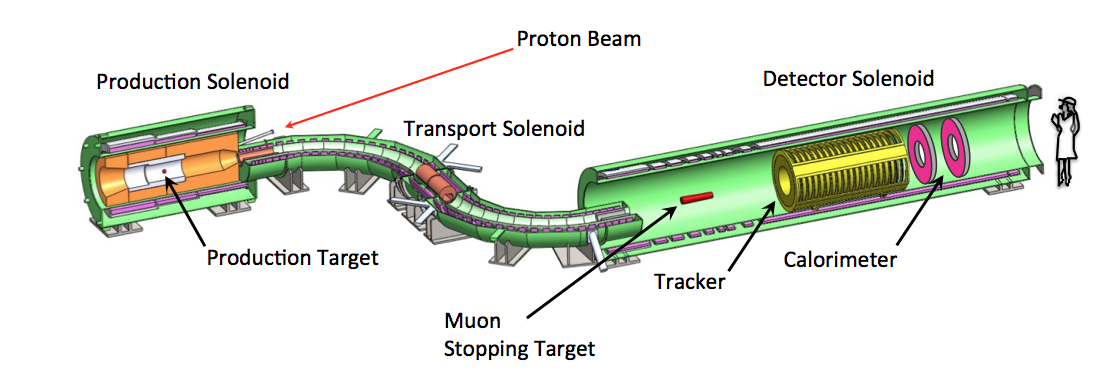
\includegraphics[width=0.8\textwidth]{Images/Mu2eDetector.png}
    \caption{Apparatus used in the Mu2e experiment}
    \label{Mu2eApparatus}
\end{figure} 

\section{Tracker}
The main purpose of the tracker is to measure the momentum of electrons with energies above 53 MeV. To accomplish this, the tracker will consist of 20,736 Mylar straw tubes ranging in length from 334 mm to 1174 mm with diameters of 5 mm. These straws will be arranged into planes which when combined form the tracker (Figure \ref{trackerSolenoid}).

\begin{figure}[htp!]
    \centering
    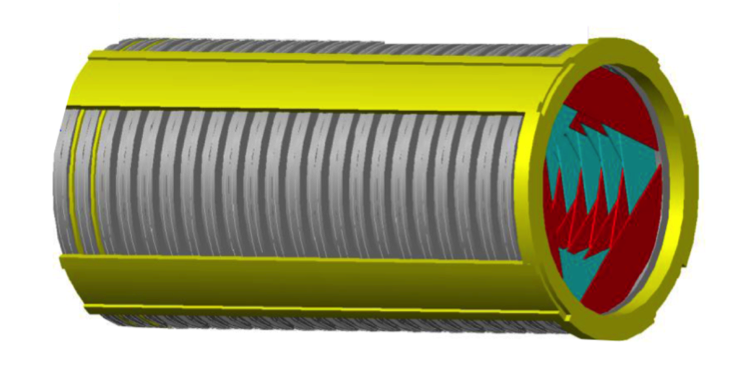
\includegraphics[width=0.55\textwidth]{Images/trackerSolenoid.png}
    \caption{Tracker solenoid.}
    \label{trackerSolenoid}
\end{figure} 

Each straw is a drift chamber such that when a particle passes through the straw, it will ionize molecules in the gas resulting in a current on the wire. This current is then passed through the straw electronics which shapes the signal to produce a voltage waveform.

By integrating the waveform from the Analog-to-Digital Converter (ADC) output, it is possible to obtain an estimate of the deposited energy. The deposited energy can then be used to differentiate particle species. In addition to muons, a major source of accidentals in the detector will be due to protons produced by nuclear breakup from muon capture. Since the average proton produced will deposit significantly more energy (roughly one order of magnitude greater) than the electrons, computing the energy from the ADC output will play a major role in differentiating these particles.

\section{Simulations}
Currently, the Mu2e collaboration has produced simulations of the tracker and the corresponding electronics. These  simulations assume the electronic response is well-approximated a high-pass RC filter followed by a low-pass CR filter to produce a voltage waveform of the form.

\begin{equation}
   V (t) = \frac{t}{\tau^2} e^{-t / \tau}
 \end{equation} 
where $V$ has been normalized. This potential is then digitized by an ADC. A sample output is shown in Figure % \ref{SampleWaveform}. 

FIXME : IMPROVE THIS

\section{Tracker Prototype}
To study the straw electronics, a prototype of the tracker has been used.
\begin{figure}[htp!]
    \centering
    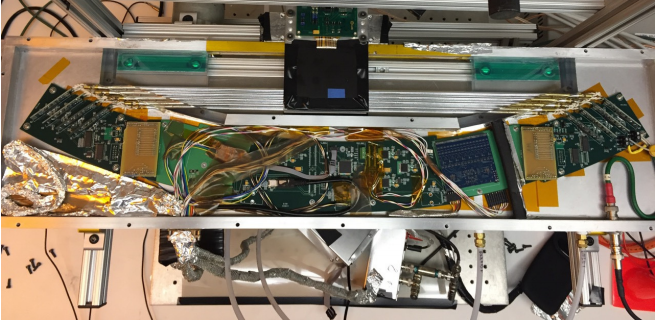
\includegraphics[width=0.55\textwidth]{Images2/prototype.png}
    \caption{Prototype of the Mu2e tracker.}
    \label{prototype}
\end{figure} 
The prototype consists of eight straws which together make up a subset of one panel (Figure \ref{prototype}). With this setup radioactive sources were pointed at the straws to produce signals that mimic what will be seen in the actual experiment. With this data we can verify and measure properties of the straw electronics, and in addition update and tune the current simulations.

 %At lower voltages the output of the simulations appear correct. However, at higher voltages corrections are clearly needed. In addition, several other electronic parameters appear to be different than the values currently implemented in the simulation. 

\section{Purpose}
The goal of the work described in this paper is twofold. First, we study the output of the tracker prototype and reconcile several results with the simulation. Second, we develop algorithms to efficiently reconstruct the energies from the waveforms. This will be key in differentiating hits from electrons and protons and determining a particle's identity.


 % Introductory chapter
% ch:relatedwork
%!TEX root = AllegThesis.tex
%
% $Id: ch02_relatedwork
%
\chapter{Tracker Electronics Corrections}\label{ch:trackerelectronics}

In the summer of 2015, the Mu2e group obtained a prototype of a subset of the tracker. This provided some of the first opportunities to study the straw electronics response and compare it to simulations. In this chapter, several of these measurements using the ADC output are presented, many of which have been used to compare to and update the current Mu2e simulations.

\section{Low Energy Waveforms}

When a particle passes through a straw, it ionizes charge which then produces an impulse of current on the straw wire. This current is then shaped by the electronics and digitized by the ADC. Although, the shaping is in reality much more complex, it has been modeled as a simple RC CR circuit. With this assumption, a signal of the form 
\begin{equation}
	V(t) = V_0 \frac{t}{\tau^2} e^{-t / \tau}
	\label{eq:base1}
\end{equation}
\begin{figure}[htp!]
    \centering
    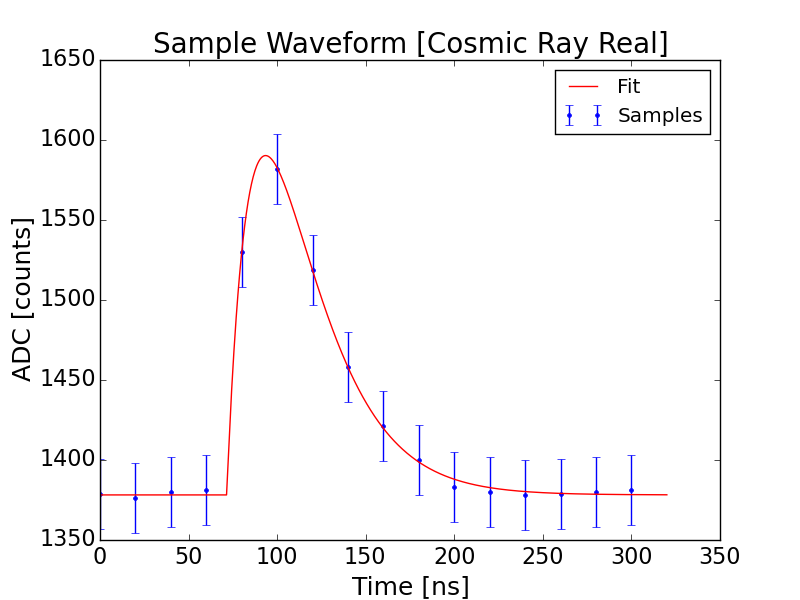
\includegraphics[scale=0.5]{Images2/sampleWaveformCosmic.png}
    \caption{Sample waveform of cosmic muon from ADC output.}
    \label{fig:sampleCosmic}
\end{figure} 
is obtained, where $\tau$ defines the shaping time, and $V_0$ is constant which depends on the amount of energy deposited by a given particle. A sample waveform is shown in Figure \ref{fig:sampleCosmic} with a fit to this model superimposed. 

The source used to produce this waveform was
cosmic-ray muons. These muons are classified as minimum ionizing particles (mip's). Consequently, they should have a similar $dE/dx$ and thus deposit energy in a similar manner to electrons in the actual experiment.

Qualitatively, there is good agreement between this simple model and the prototype waveforms. This provides some validation to the electronics model in the simulations. ???

\section{Shaping Time}
In the current simulations, the default value for the shaping time has been fixed to $25$ ns, a value based on prior SPICE simulations. To more finely tune this parameter an Iron-55 source used. Fe-55, emits photons which have a very precise-value for their energy, and produce a single cluster of ionizations. This local cluster of ionizations well-approximates a current impulse. This is in contrast to massive particles which produces a path of ionizations that reach straw wire over a range of time. By fitting Equation \ref{eq:base1} to Fe-55 waveforms, with $\tau$ as a free parameter we can determine a more precise value for this parameter. Figure ... shows the distribution of this fit parameter, with a peak near $22$ ns and a reasonable small spread. This value has been added as the default to the Mu2e simulations.

\section{ADC Gain and Noise}

\subsection{ADC Gain}

\begin{figure}[htp!]
    \centering
    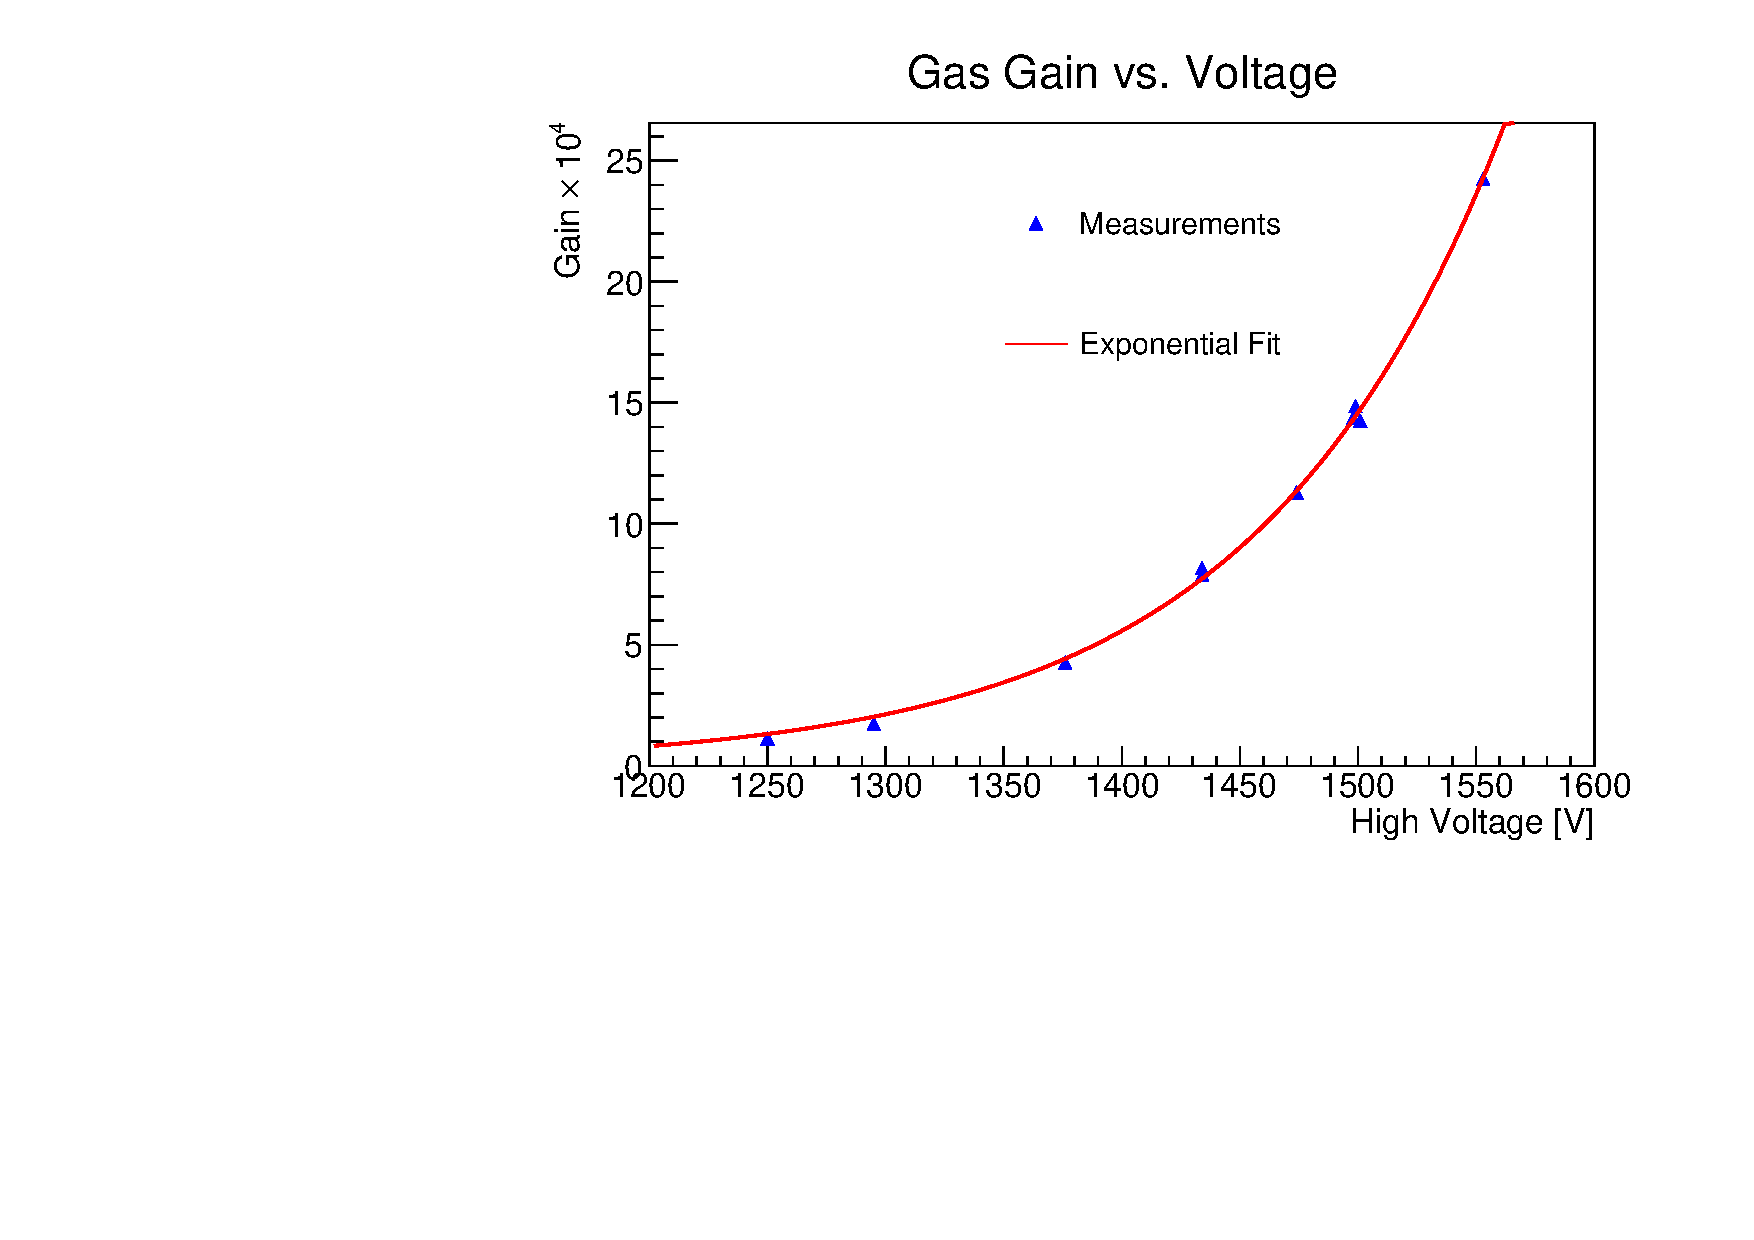
\includegraphics[scale=0.5]{Images2/gasGainVsVoltage.pdf}
    \caption{Gas gain as a function of high voltage.}
    \label{fig:gasGain}
\end{figure} 
When the current impulse reaches the wire, it is not only shaped but also magnified by a preamp. This corresponds to a vertical scaling of the ADC waveform. 
%A part of the amplification results from the chain reaction of ionizations that occur in the gas as the incident particle pass through the straw. A second amplification occurs purely from amplifiers contained in the straw electronics. The first amplification (which we define as the gas gain) has been found through previous measurements to be related to the high voltage across the straws. This relationship is shown in Figure \ref{fig:gasGain}. 
We can measure this amplification (defined to be the electronics gain) once again by using Fe-55 data. The advantage to using Fe-55 is that the 5.9 keV peak in it's energy spectrum is well-defined in Geant4, which can easily be simulated in Mu2e Offline. 

Given the energy deposited by a single photon ($E_{\gamma}$) from the Fe-55 source and knowing computing the energy per ionization ($E_{ionization}$) using Geant4 then the voltage outputted by the ADC is given by
\begin{equation}
	 \frac{E_{\gamma}}{E_{ionization}} \times {Gain_{gas}} \times Gain_{electronics} = V_{ADC}
	 \label{eq:electronicsGain}
\end{equation}
The gas gain ($Gain_{gas}$) is defined to be the scaling resulting from the chain reaction of ionizations that occur in the gas as the incident particle pass through the straw. This amplification has been found through previous measurements to be related to the high voltage across the straws (shown in Figure \ref{fig:gasGain}). 

By measuring energy spectrum of the Fe-55 waveforms using the prototype, we can compute $V_{ADC}$ which corresponds to the voltage at the peak and scale this value to find the corresponding electronics gain.

\subsection{ADC Noise}

By studying the width of the peak, we can also estimate the noise in the signal. Sources of noise affecting the ADC output, include gain variation, smearing from the ADC sampling rate, and electronics noise. This noise will increase the variation of the ADC output which will widen the width of the peak. We can estimate the amount of noise by varying the noise in the simulation to match the width seen in the prototype data. Doing this, the noise was measured to be approximately 8 mV. Figure ... shows a comparison of the spectrums for Fe55 using both the prototype and simulations. After tuning the electronics gain and noise, the spectrum for the 5.9 keV peak match. On a side note, below the 5.9 keV there is less agreement between the simulations and data. This is because Geant4 currently does not currently simulate the 2.9 keV escape peak.

\section{Threshold Gain and Noise}

In the straw electronics a threshold is applied so that only signals of a certain amplitude are outputted by the ADC. This is important for reducing the amount of low energy noise from signals of interest. Theoretically, the threshold should form a step-function in acceptance, eliminating all signals below the threshold while accepting all signals above. Due to noise this response is in reality much more smooth. To measure this, the Iron-55 spectrum was measured at two different thresholds (Figure \ref{fig:peakMinusPedThresh}). The ratio of these two spectrums produces precisely the threshold response (Figure \ref{fig:relativeRates}).

\begin{figure}[htp!]
    \centering
    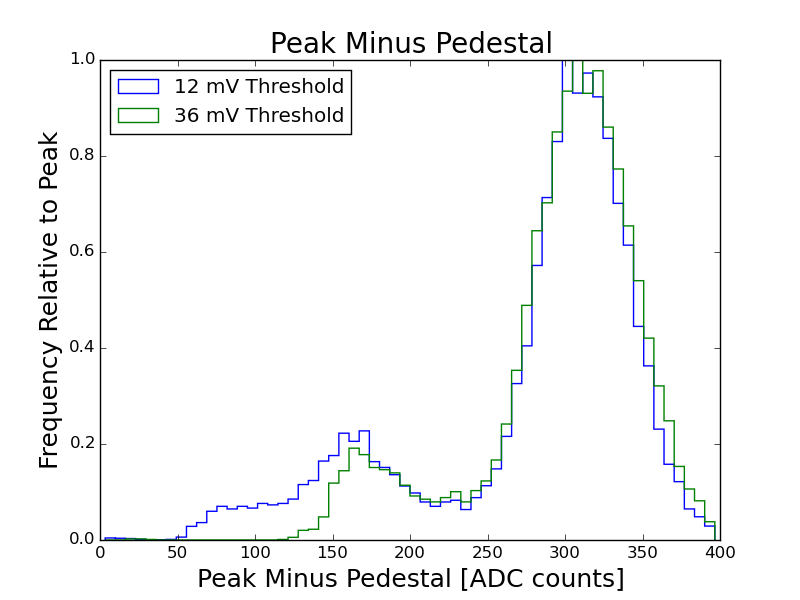
\includegraphics[scale=0.5]{Images2/peakMinusPedThresh.png}
    \caption{Peak minus pedestal for 12 mV and 36 mV thresholds.}
    \label{fig:peakMinusPedThresh}
\end{figure} 
\begin{figure}[htp!]
    \centering
    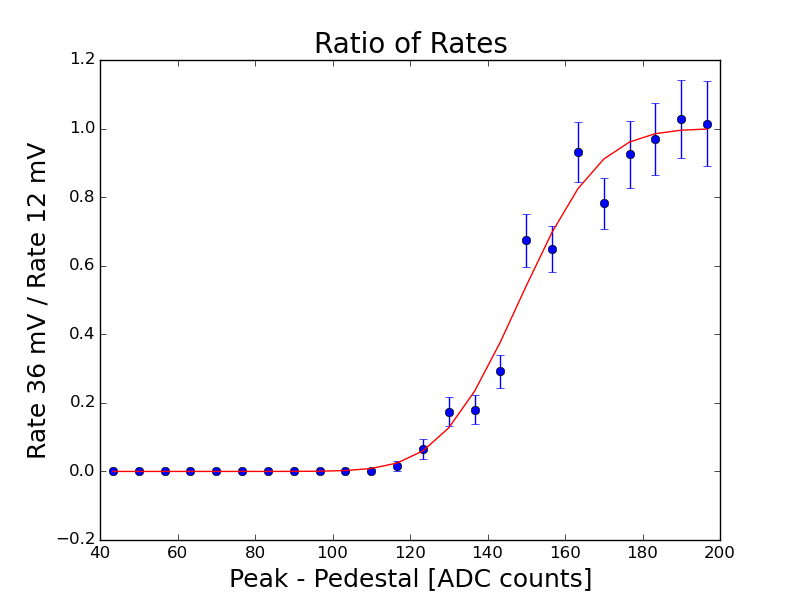
\includegraphics[scale=0.5]{Images2/relativeRates.png}
    \caption{Ratio of peak minus pedestal for 12 mV and 36 mV.}
    \label{fig:relativeRates}
\end{figure} 


As expected, the ratio forms a smooth step function. This data was fitted to the functional form
\begin{equation}
    g(x; a,b) = \frac{\text{erf}\left( a(x - b) + 1 \right)}{2}
\end{equation}
Note that $a$ defines the threshold which the ratio is $1/2$. $b$ in the other hand defines the spread in the function, and hence provides a estimate for the noise in the threshold channels.



\section{Preamp Saturation \label{sec:preampSaturation}}
The straw electronics contains a preamp. At voltages this component is useful for amplifying the signal. However, for higher voltages the preamp saturates. Measuring the levels at which saturation occur are important for reducing crosstalk between straws. In otherwords, if the saturation level is too high (which can result from proton background), signals in one straw may become large enough that the corresponding signals induced in neighboring straws may overwhelm signals of interest. 

Like in the previous studies an Fe-55 source was used. %Given the energy deposited by Fe-55 we can compute the corresponding number of ionizations. This in turn can be used to compute the charge deposited on the straw wires, which is directly proportional to the current and hence to the voltage measured in the ADC output. The full relationship between the energy deposited and the resultant charge on the straw is shown in Equation \ref{eq:electronicsGain}.
Given the High Voltage, with Equation \ref{eq:electronicsGain} we can compute an estimate for the voltage measured with the ADC in the linear regime. Thus, for voltages in this linear region we expect this estimate to match what is the value measured with the protype. However, by comparing this estimate over a wider range of voltages we can determine where the preamp response becomes nonlinear and saturates.

\begin{figure}[htp!]
    \centering
    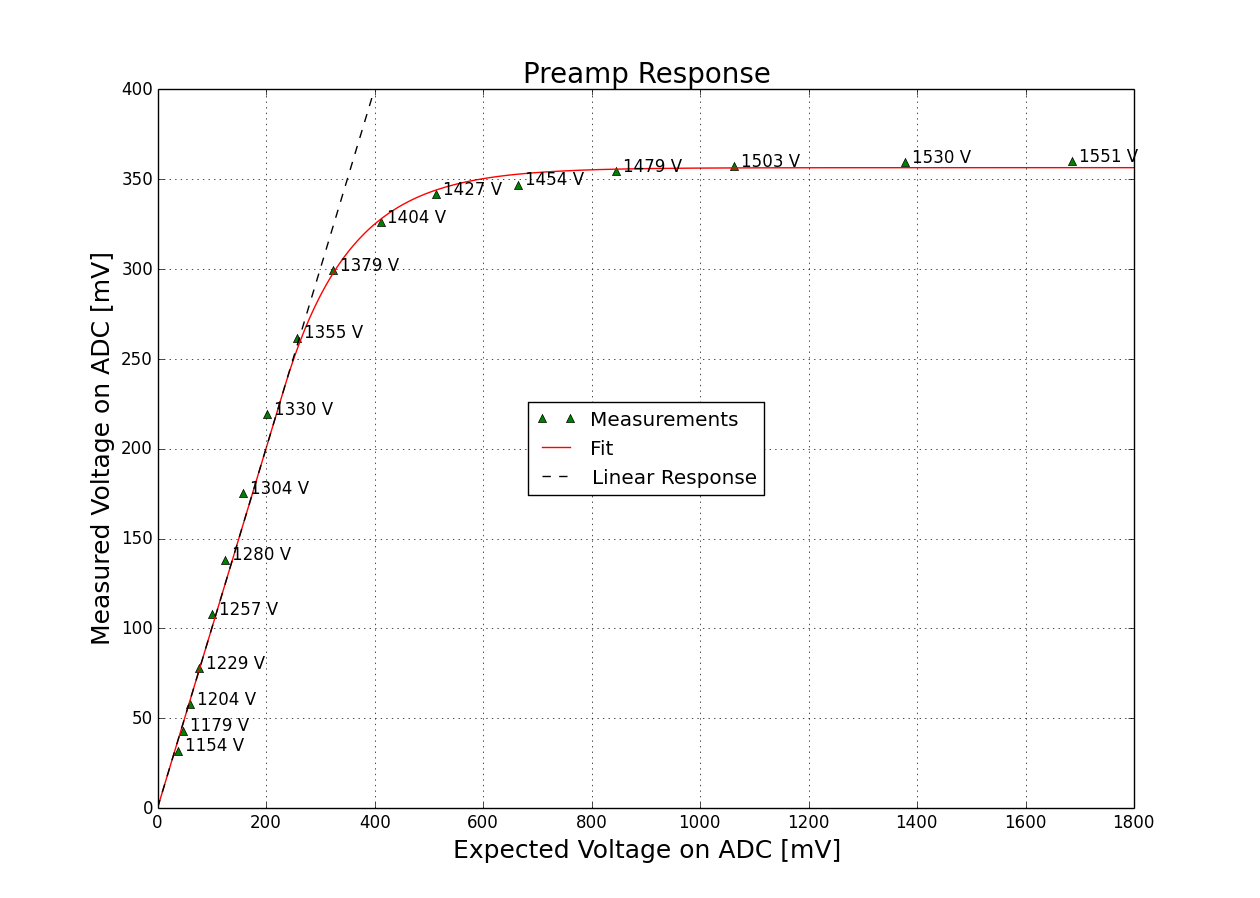
\includegraphics[scale=0.4]{Images2/preampResponse.png}
    \caption{Preamp response over a range of high voltages.}
    \label{fig:preampResponse}
\end{figure} 

Figure \ref{fig:preampResponse} shows the measured voltage versus the computed voltage over a wide range of frequencies. This response was fit to the model 
%Figure ... shows the relationship between the ADC output versus the deposited charge. As expected, for lower voltages the response is clearly linear. By fitting a line to the linear regime, the scaling factor between the resultant voltage from the ADC and the deposited charge was found to be ...
%Rescaling the charge by this value, Figure ... shows the preamp response purely as a function of voltage. The response was fit to the model
\begin{equation}
	f(V; V_{sat}, V_{max}) = \begin{cases} 
		V & V < V_{sat} \\
		V_{sat} + (V_{max} - V_{sat}) e^{-\frac{V - V_{max}}{V_{sat - V_{max}}} } & V \geq V_{sat} \\
		\end{cases} 
\end{equation}
where $V_{sat}$ is the threshold at which the preamp response becomes nonlinear and $V_{max}$ is the maximum response for any voltage. 

The resultant fit parameters were $V_{max} = 356 mV$ and $V_{sat} = 234 mV$, which have been incorporated into the Mu2e simulation. The dynamic range of the preamp is $1500 mV$ which is significantly greater than $V_{max}$. In Section \ref{sec:sat} methods are developed to recover much of the dynamic range from the ADC waveforms. 

\section{High Energy Corrections}

All the studies so far have been succesfully implemented into Mu2e Offline. For this final study significant process has been made. However, further work is still needed before it can be incorporated the Mu2e framework.

Prior to the studies using the prototype all waveforms were predicted to be of the form in Equation \ref{eq:base1}. With the prototype at Low Energies this function appeared to hold true. However, for higher energy pulses an undershoot begins to appear (Figure ...). Most of the waveforms resulting from conversion lie in the lower energy regime. This undershoot is prevalent in many proton signals. Depending on the decay time of this undershoot, it is possible for this additional feature to overwhelm a following conversion electron signal. In other words, the undershoot will place limits on the dead time of the ADC ???

In addition, the undershoot will restrict possible energy reconstruction methods. In particular, the current method used to reconstruct the energy deposited by a waveform involves summing the ADC values and subtracting the pedestal. However, for waveforms with large undershoots, the estimated energy will be severely reduced. Thus other methods, such as computing the difference between the peak value and the pedestal or a fitting method must be used. 

To model this extra feature a current waveform is added to Equation \ref{eq:basefit} of the form 
\begin{equation}
	U(t;t_0,n,\xi) = - U_0 \left( \frac{t - t_0}{\xi n} \right)^n e^{-(t - t_0 - \xi n)/\xi }
\end{equation}
The total waveform is thus $V(t) + U(t;t_0,n,\xi)$. The functional form of $U(t;t_0,n,\xi)$ is very similar to a negated version of $V(t)$, with some subtle changes in the parameters:
\begin{itemize}
\item Similar to $\tau$ in $V(t)$, $\xi$ describes the decay time back to pedestal. 
\item $t_0$ defines the time at which the undershoot first appears with respect to the start in $V(t)$.
\item Normalization is chosen so that the minimum occurs at $U_0$. For $V(t)$, normalization was chosen so that the integral of $V(t)$ from zero to infinity was $V_0$.
\item $n$ defines the power of the term which is polynomial in $t$. Consequently, the minimum of $U$ occurs at $t = \xi n$. For comparison, the maximum of $V_0$ is constrained to $t = \tau$.
\end{itemize}


An example waveform is shown in Figure ... This method reasonably models the general shape of the waveform and consequently could be incorporated into energy reconstruction methods (see Chapter \ref{ch:implem}). However, it is not so clear how best to implement this model into the simulations. In the simulations for each hit subsets of the charge (called hitlets) are individually shaped and the resultant waveforms are summed linearly. The undershoot though is a inherently time-dependent effect and does not scale linearly with charge. At the moment, the candidate implemention is to add these small undershoots to each hitlet and like before simply sum up all these individual response. This is not without drawbacks, and has yet to be fully implemented (What are the drawbacks???). For more precise simulations a more complex model of the straws electronics will be necessary.

pixel/mu2e/allruns/lbl-cosmics


 % Background chapter
% ch:thework
%!TEX root = AllegThesis.tex
%
% $Id: ch04_implementation.tex
%
\chapter{Energy Reconstruction}\label{ch:implem}

In this chapter we present methods for reconstructing the energies deposited by particles using ADC waveform measurements. This analysis is key for differentiating electrons from sources of background, most notably protons.

\section{Methodology}

\begin{figure}[htp!]
    \centering
    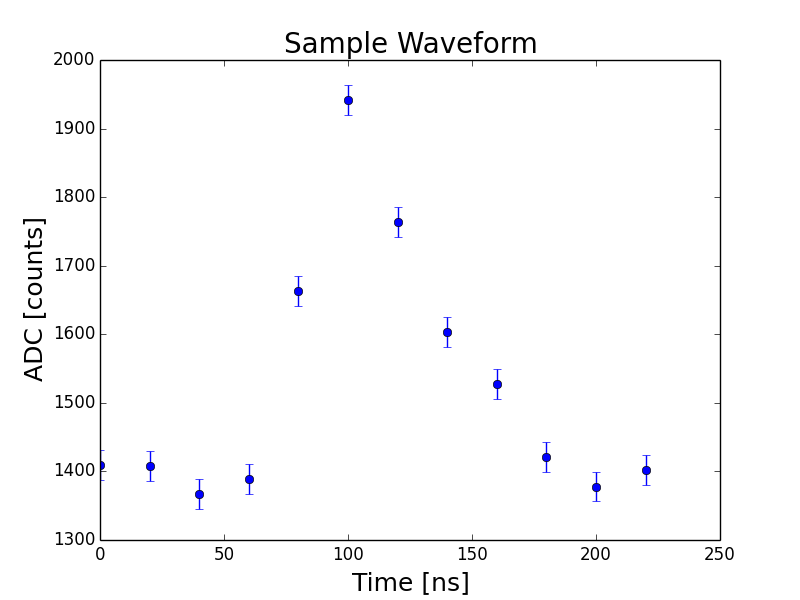
\includegraphics[scale=0.5]{Images2/sampleWaveform.png}
    \caption{Sample waveform of ADC output.}
    \label{fig:sampleWaveform}
\end{figure} 
To develop the following methods, 500 events of conversion electrons with full hit background overlay (accidental signals resulting from unavoidable processes related to stopping muons in aluminum) were simulated using Mu2e Offline. This provides the most accurate simulations of the output of the ADCs to date. Each hit is recorded as a 240 ns interval of output from the ADC. Samples are measured at a fixed clock frequency of 50 MHz. Hence, twelve samples are measured for a given hit. Using a 12-bit ADC, each sample lies in the range of 0 to 4095 counts. Four of these samples, called presamples, are measured immediately prior to the signal crossing threshold. A sample waveform is shown in Figure \ref{fig:sampleWaveform}. 


\subsection{Monte Carlo Truth Energy}
For comparison, a variable provided in the Mu2e simulations, known as the Monte Carlo truth energy (MC energy) has been used. The MC energy is defined to be the total energy deposited on a straw over the interval of a given hit. In many cases the MC energy describes precisely the value we hope to compute. However, for a small portion of cases in which two or more particles go through the straw within the same 240 ns period, this value will be higher than the computed energy of a hit. A frequency plot of the MC energies of the electrons and protons is shown in Figure \ref{mcenergydistributions}. Electron hits can be separated by cutting on the deposited energy. Note that for any cut in energy, it will be impossible to completely differentiate protons and electrons due to the overlap in energies.

\begin{figure}[htp!]
    \centering
    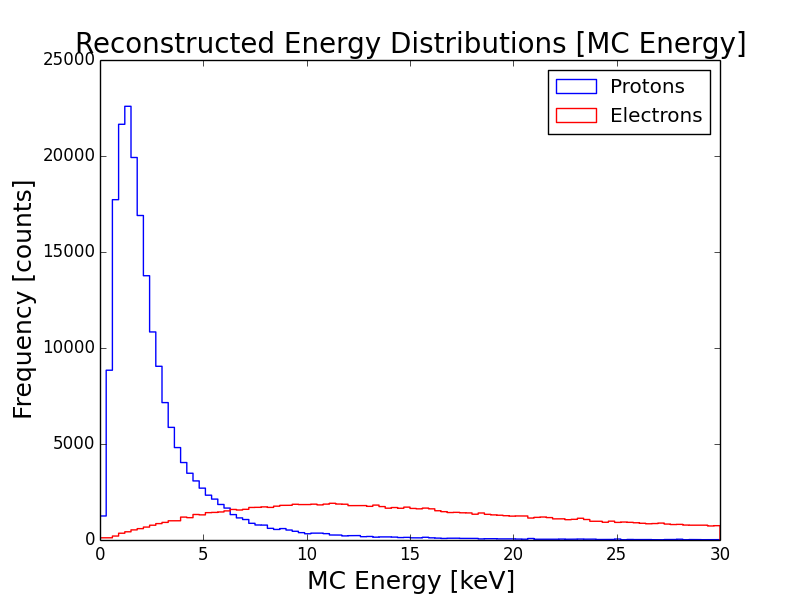
\includegraphics[width=0.6\textwidth]{Images2/mcenergy.png}
    \caption{MC energy frequency distributions for electrons and protons.}
    \label{mcenergydistributions}
\end{figure} 


\subsection{Sum Method}

The current method in the Mu2e software used to compute the energy of a hit is to simply sum the values of the ADC and subtract the mean of the presamples. This method has already been succesfully implemented in the Mu2e simulations and can therefore be considered the baseline method. In other words, the method developed over the following sections must differentiate protons and electron hits at least as well as the sum method.


\subsubsection{Methods of Comparison}
To compare the various methods, a purity-efficiency plot is used. For any method, the purity-efficiency plot contains a comparison between the power of rejection of protons and the acceptance rate of electrons for various cuts in energy. For example, the purity-efficiency curves for the sum method and MC energy data are shown in Figure \ref{rejectionPlotSumAndMCenergy}. Conceptually, it is easy to see that a "better" method's rejection curve will lie above the purity-efficiency curve of a "poorer" method. Therefore, this type of plot will be used as the main tool in comparing the success of different methods. %In addition, since there is a gap betwen the two curves, this comparison shows that improvement over the sum method is possible.

\begin{figure*}[ht!]
    \centering
    \makebox[0pt]{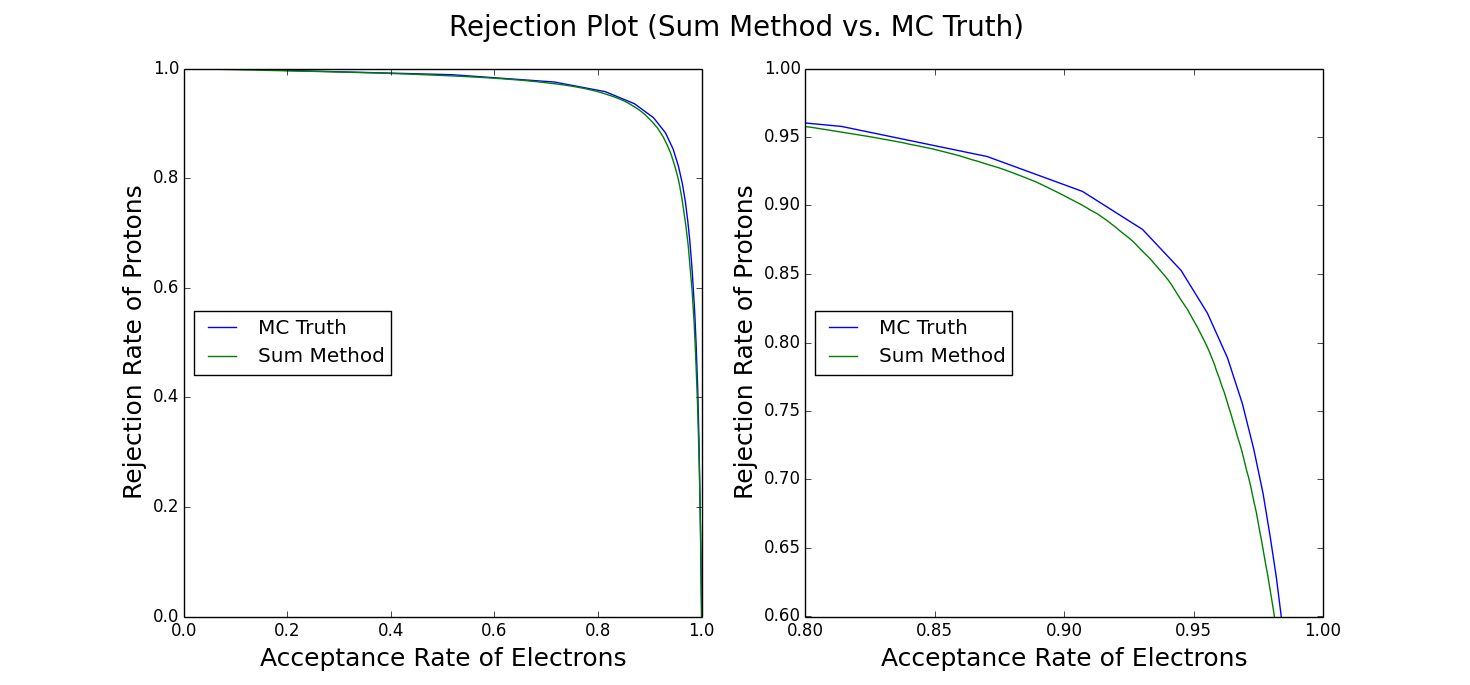
\includegraphics[scale=0.5]{Images2/rejectSumMC.png}}
    \caption{Purity-efficiency curves for sum method and MC energy.}
    \label{rejectionPlotSumAndMCenergy}
\end{figure*} 





\section{Base Fit Method}
 When a particle deposits charge on a straw wire it produces an impulse of current, which is then shaped and digitized by the straw electronics. This shaping can be well-approximated by the composition of an RC and CR filter (Figure \ref{RCCRCircuit}).
%the potential outputted by the ADC would appear as a simple step function. To amplify the signal while controlling the amount of noise a high-pass RC filter followed by a low-pass CR filter have been added to the design. 
\begin{figure}[htp!]
    \centering
    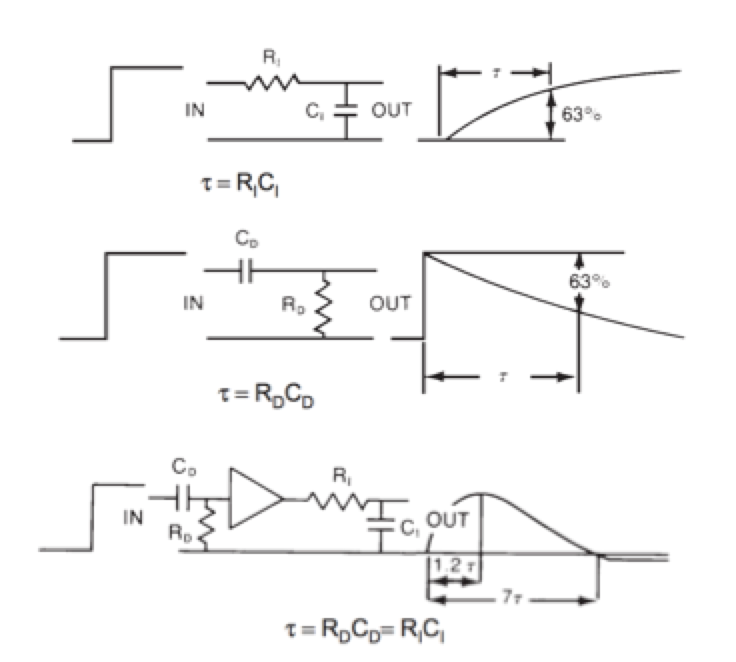
\includegraphics[width=0.6\textwidth]{Images/RCCRCircuit.png}
    \caption{The top diagram shows the effect of an RC circuit on a charge step function, the center shows the effect of a RC circuit on a charge step function, while the bottom diagram depicts the effect of combing these two circuits.}
    \label{RCCRCircuit}
\end{figure} 
This produces a signal of the form 
\begin{equation}
  V(t) = \frac{t}{\tau^2} e^{-t / \tau}
\end{equation}

with shaping time $\tau$.
 For times $t$ less than zero, the function is set to zero.

Qualitatively, most of the hits have this form. However, the waveform can vary in three ways:
\begin{enumerate}
\item The signal's magnitude $(A)$
\item The time at which the signal begins with respect to the 240 ns interval ($t_0$)
\item The initial voltage when the signal begins ($p_0$)
\end{enumerate}
The corresponding functional form is
\begin{equation}
  V(t) = A \frac{(t - t_0)}{\tau^2} e^{-(t - t_0) / \tau} + p_0
  \label{eq:basefit}
\end{equation}.
Note that even though all three of these parameters are necessary to establish the fit, since 
\begin{equation}
  E_{deposited} \propto \int_{0}^{\infty} V(t) - p_0 \text{ } dt = A
\end{equation}
 the energy deposited on the wire is simply proportional to $A$. Hence, after a fit has been applied to a hit, no other computations are necessary to establish the particle's relative energy.

Fitting the ADC data to Equation \ref{eq:basefit}
and extracting the energy from the fit parameter $A$ defines the base fit method. A sample waveform fitted using this method is shown in Figure \ref{fig:sampleBase}.

\begin{figure*}[ht!]
    \centering
    \makebox[0pt]{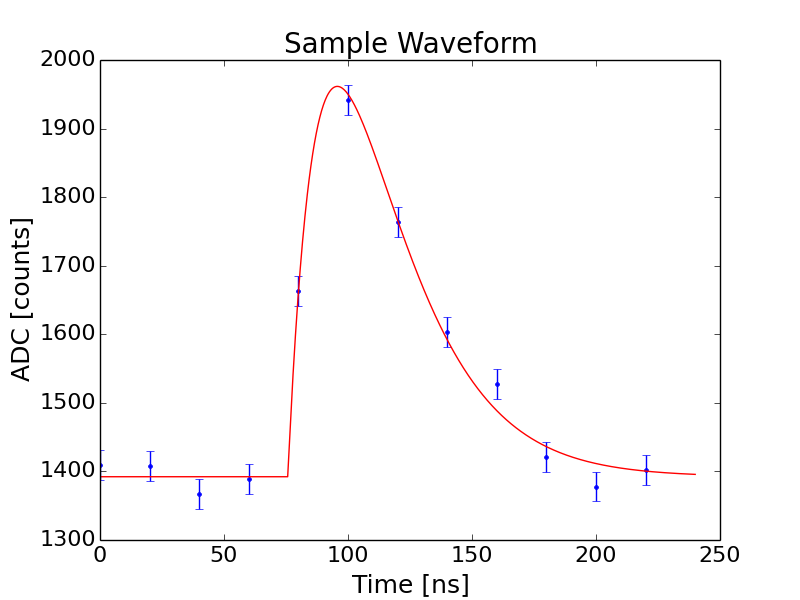
\includegraphics[scale=0.5]{Images2/sampleBase.png}}
    \caption{Sample waveform fitted using basefit method.}
    \label{fig:sampleBase}
\end{figure*} 



%For comparison, consider the plot in Figure \ref{baselineChiSquareDistribution} of the reduced chi-square values of the electron hits fit by this curve. The distribution is centered at one as we would expect. In addition, as shown in Figure \ref{rejectionPlot} this method is better at differentiating electrons and protons than the basic sum method.


%\begin{figure}[htp!]
%    \centering
%    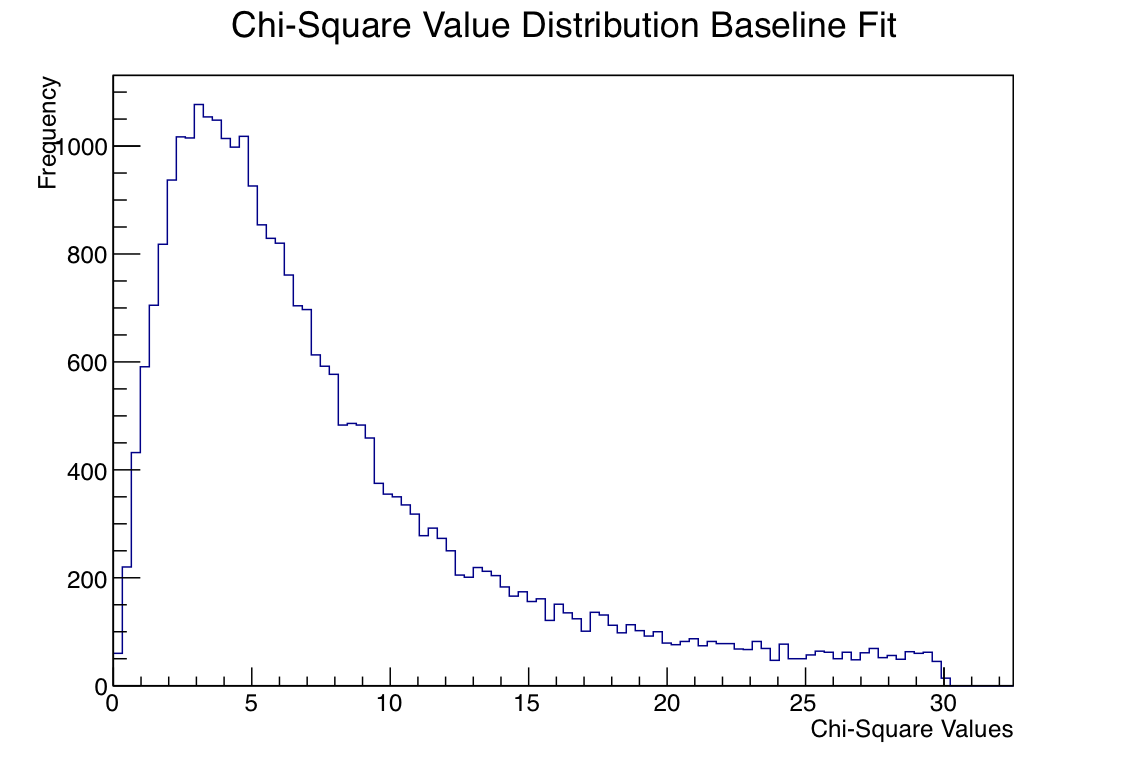
\includegraphics[width=0.6\textwidth]{Images/baselineChisquared.png}
%    \caption{ Chi-squared distributions for the baseline fit method.}
%    \label{baselineChiSquareDistribution}
%\end{figure} 


%For comparison, the reconstructed energies is plotted against the corresponding MC energies. 


%\begin{figure*}[ht!]
%    \centering
%    \makebox[0pt]{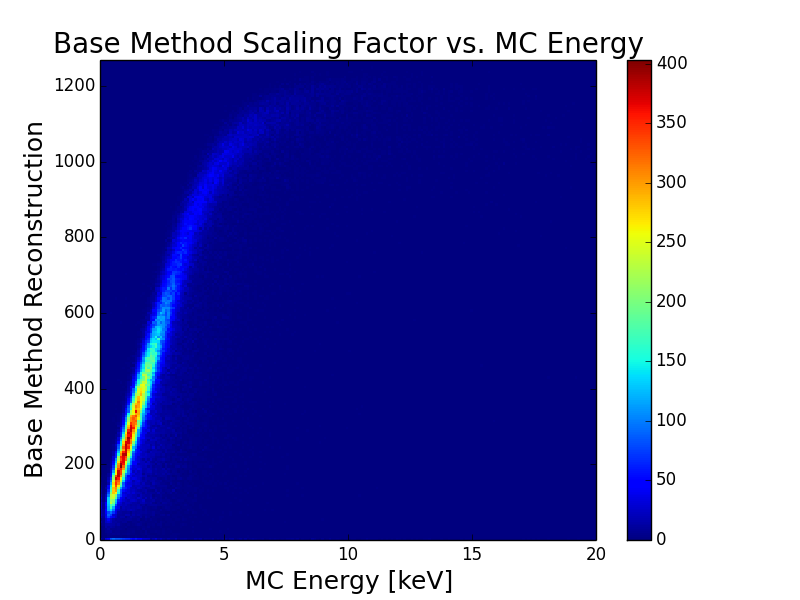
\includegraphics[scale=0.5]{Images2/baseVsMC.png}}
%    \caption{Reconstructed energies using basefit method versus MC energies.}
%    \label{fig:sampleBase}
%\end{figure*} 




For comparison, a frequency plot of the reconstructed energy distributions for the protons and electrons is shown in Figure \ref{fig:recoEnergyFunc1}. From this graph, this fit is quite strong at separating protons and electrons at the 3 KeV energy cut. In addition, it is also apparent that the fit breaks down at higher energies. This is a consequence of saturation in the preamp as discussed Section \ref{sec:preampSaturation}.
 \begin{figure}[htp!]
    \centering
    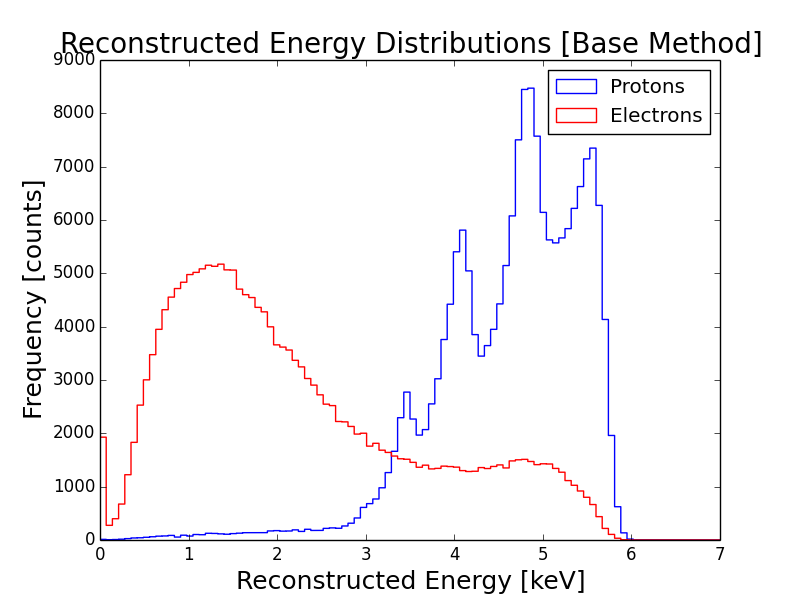
\includegraphics[width=0.6\textwidth]{Images2/base.png}
    \caption{Reconstructed energies using base fit method.}
    \label{fig:recoEnergyFunc1}
\end{figure} 

Clearly, this method is able to differentiate electrons to some degree. However, significant improvements are needed to outperform the sum method. This can be seen from purity-efficiency plot at the end of the chapter.

\section{Convolved Fit Method}
One underlying assumption used in the basefit model is that when a particle passes through a straw it produces a delta function of current on the corresponding wire. However, depending on where in the straw the electron or proton passes the corresponding charge on the wire may be deposited with some spread in time (shown in Figure \ref{fig:hitletTimes}).

\begin{figure}[htp!]
    \centering
    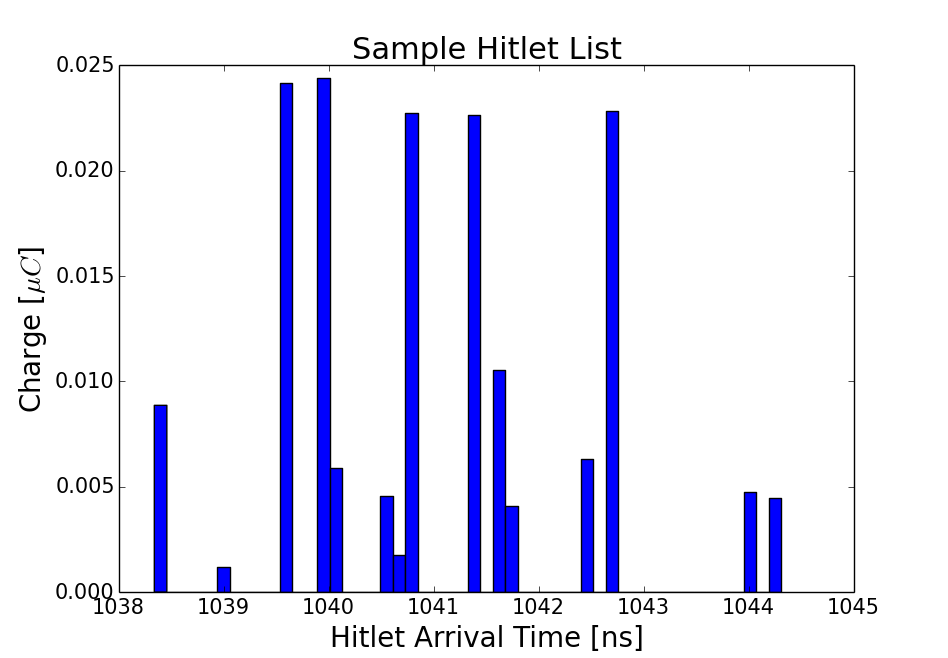
\includegraphics[width=0.6\textwidth]{Images2/hitletlist.png}
    \caption{Simulated arrival times of charges for a given hit.}
    \label{fig:hitletTimes}
\end{figure} 


Consequently, a better approximation for the output from the ADC is the base fit model convolved with a uniform distribution
\begin{equation}
    g(t) = \frac{1}{2 \sigma} \text{ for } t \in \left[ -\sigma, \sigma \right]
\end{equation}
where $\sigma$ is a free parameter defined to be half of the width of the uniform distribution.


Convolving this with Equation \ref{eq:basefit} produces 

\begin{equation}
   V \circ g =  \int_{\infty}^{\infty} V(t - t') g(t') dt' = \left. \frac{1}{2 \sigma}\left[ -e^{-t'} (t' + 1) \right] \right|_{max(\frac{t - \sigma}{\tau},0)}^{max(\frac{t + \sigma}{\tau},0)}
 \end{equation}.

 Adding in $\sigma$ as a free parameter to the fit (in addition to three base  fit parameters), we see that this new fit function is a better fit to the hit in Figure \ref{sampleConvolvedFit}.
 \begin{figure}[htp!]
    \centering
    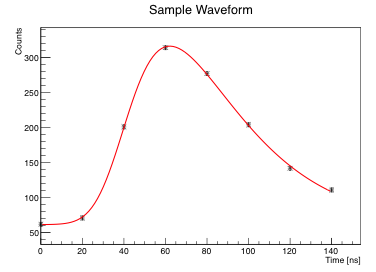
\includegraphics[width=0.5\textwidth]{Images/sampleConvolvedFit.png}
    \caption{Sample waveform with convolved fit.}
    \label{sampleConvolvedFit}
\end{figure} 
 %Consider the following frequency distribution of $\sigma$ from the various fits to events. Although many of the fits lie at $\sigma = 0$ (which is equivalent to the baseline fit model) the majority of fits have values of $\sigma$ greater than $0$, which is indicates that the adding this free parameter is beneficial.

\begin{figure}[htp!]
    \centering
    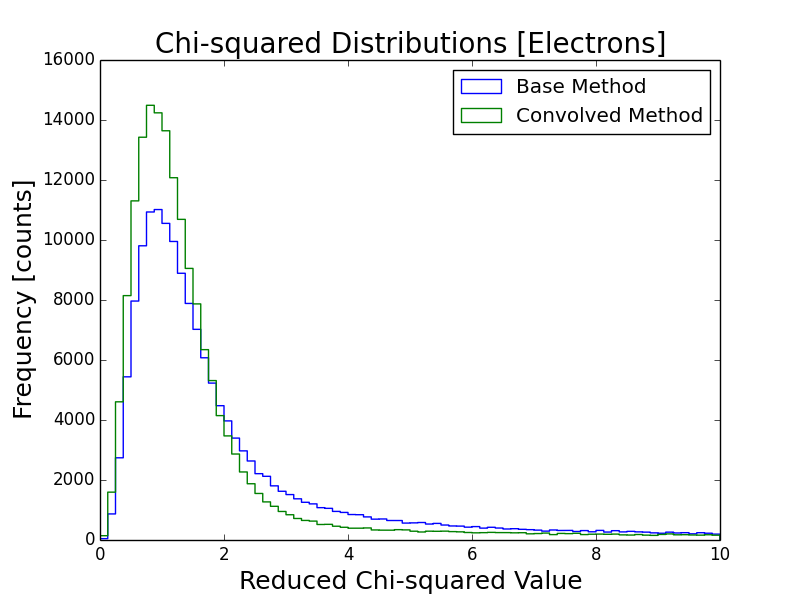
\includegraphics[width=0.6\textwidth]{Images2/chiSquareComparison.png}
    \caption{Chi-square per degree of freedom distributions for the base fit method and convolved fit method.}
    \label{fig:relativeChiSquareDistribution}
\end{figure} 
\begin{figure}[htp!]
    \centering
    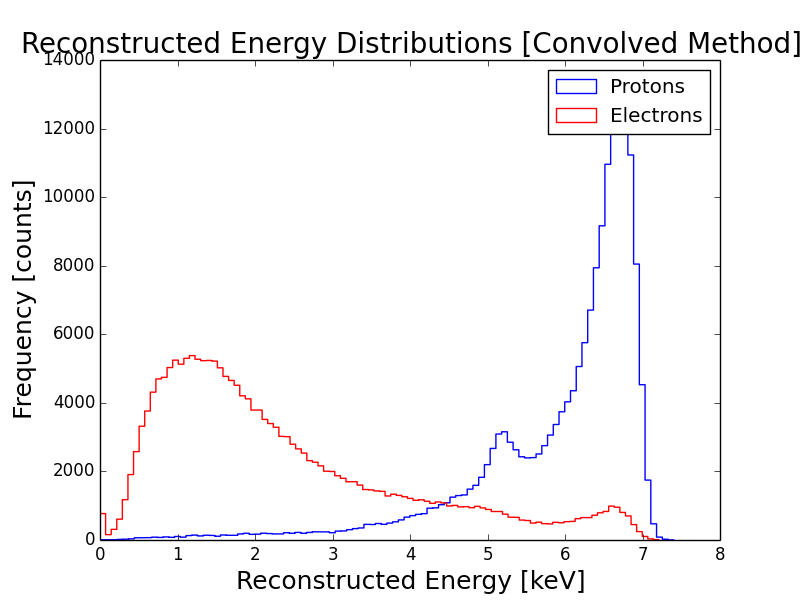
\includegraphics[scale=0.5]{Images2/convolved.png}
    \caption{Reconstructed energies using convolved fit method.}
    \label{recoEnergyFunc6}
\end{figure}


 Figure \ref{fig:relativeChiSquareDistribution} is a plot of the relative chi-squared distributions for the base fit method and the convolved fit method. Clearly, the chi-squared distribution has a much smaller tail and therefore appears to be a more accurate fit for the data.



Like for the base fit method, we can consider a frequency histogram of the reconstructed energies for the electrons and protons (shown in Figure \ref{recoEnergyFunc6}). Differentiation of electrons and protons is somewhat improved for values near 3 keV. However, there is still significant room for improvement, especially at higher energies. 

%However, for very high energies, the reconstructed proton energies appear to have two peaks. Like for the baseline fit, these somewhat unexpected results can be explained by saturation and will be taken into account in the next section.



\section{Fit Method with Saturation \label{sec:sat}}

Consider the plots in Figure \ref{fig:scalingFactVsMCenergy} of the base fit scaling factor versus the MC energy for the proton and electron hits. (Note that the scaling factor has been scaled to a rough estimate of keV.) As predicted, there is a strong linear correlation between the scaling factors and MC energies at lower energies. However, for higher energies the slope clearly begins to flatten.

\begin{figure*}[ht!]
    \centering
    \makebox[0pt]{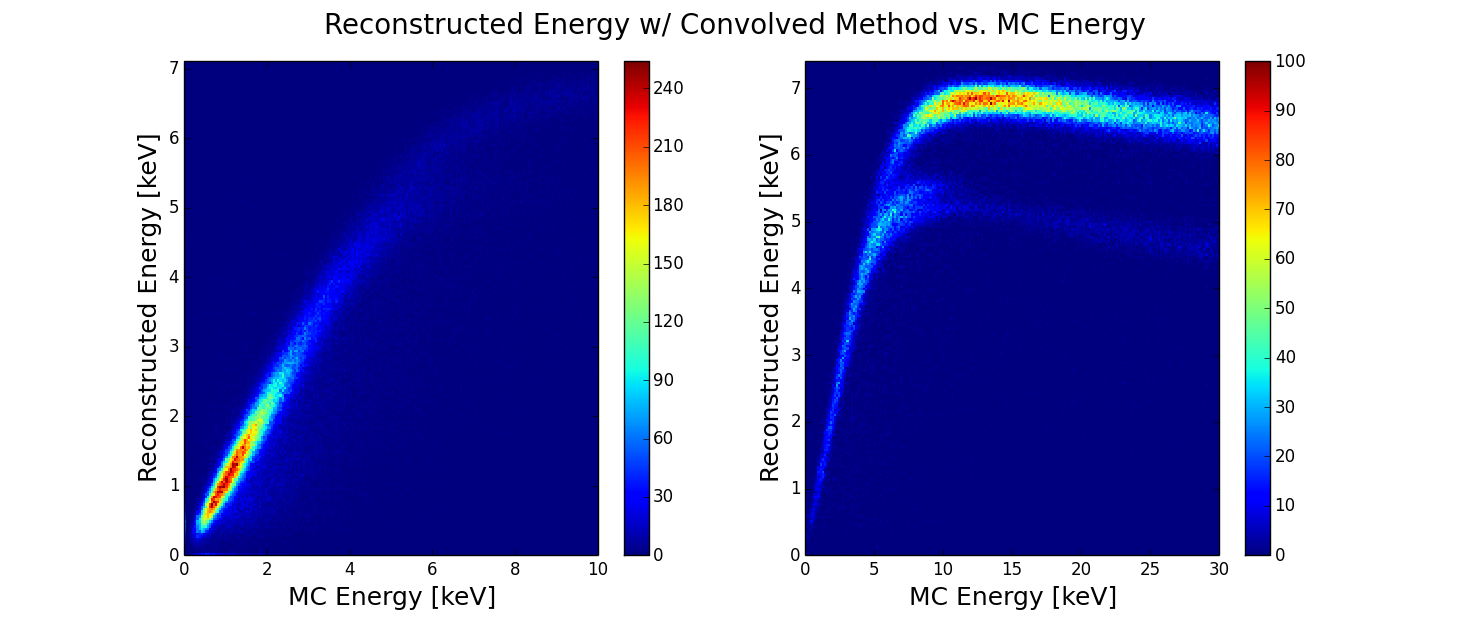
\includegraphics[scale=0.5]{Images2/convolvedVsMC.png}}
    \caption{Computed energy from ADC versus MC energy for electrons (shown on left) and protons (shown on right). Note that the energy from the ADC has been roughly scaled to units of MeV.}
    \label{fig:scalingFactVsMCenergy}
\end{figure*} 

This nonlinearity can easily be attributed to saturation. In particular, this saturation is caused by the preamp in the straws electronics, described in the previous chapter (see Figure ...). 

To improve the energy extraction, the exponential model used to fit the preamp response before, is incorporated into the fit function. The parameters corresponding to the preamp response are known from these previous measurements and thus add no new free parameters to the fit. 
\begin{figure}[htp!]
    \centering
    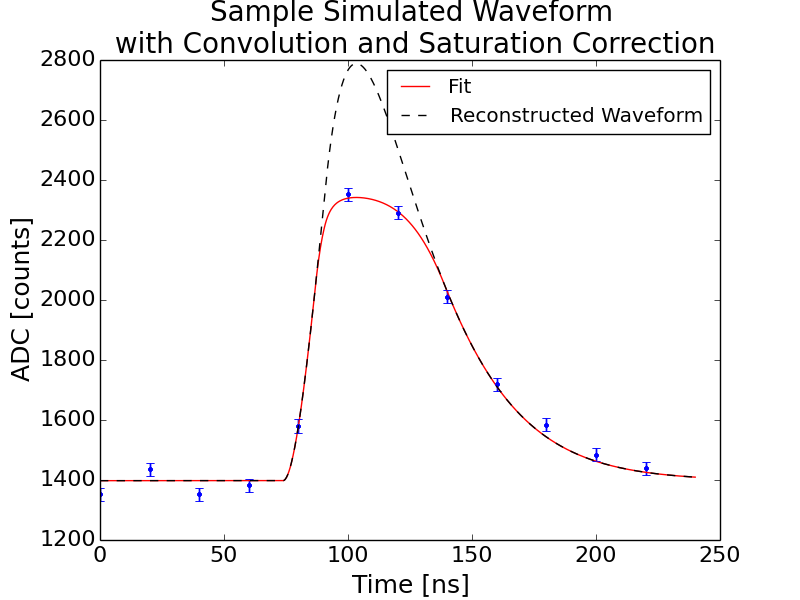
\includegraphics[width=0.5\textwidth]{Images2/recoSat.png}
    \caption{Sample waveform with convolution and saturation correction.}
    \label{fig:recoSat}
\end{figure} 

Figure \ref{fig:recoSat} is a sample waveform in which the fit incorporating saturation is very successful. Figure \ref{protonANDELectronWithTrunction} shows the reconstructed energy using the truncation fit versus the MC energy. Clearly, the response is more linear for both the electrons and protons. Note that although there is spread in the reconstructed energies for high values of MC energies, this spread is in an energy regime far beyond the energy cut value of 3 keV.

\begin{figure}[htp!]
    \centering
    \makebox[0pt]{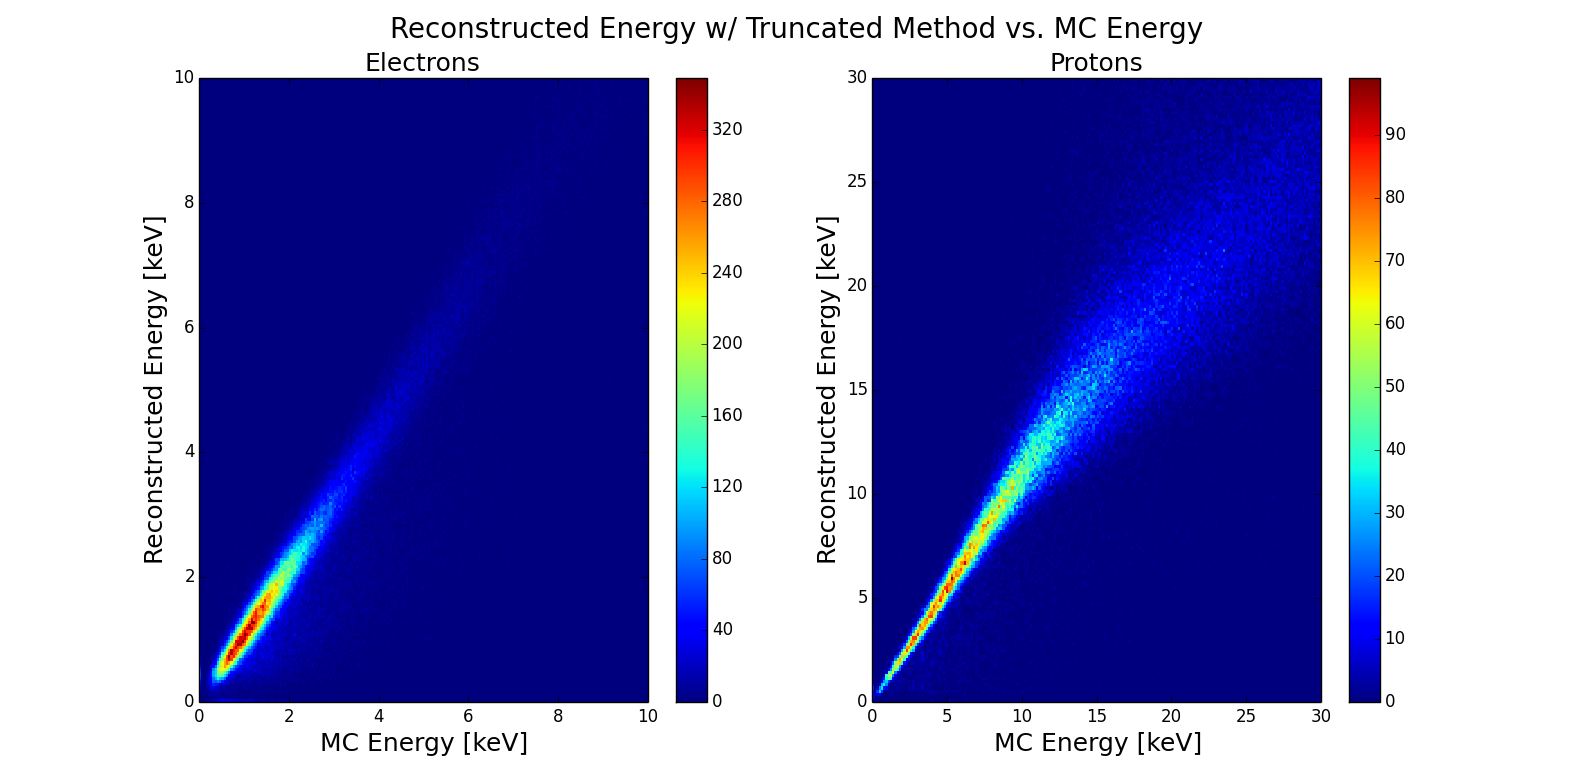
\includegraphics[scale=0.5]{Images2/truncatedVsMC.png}}
    \caption{Reconstructed energies using truncated fit method versus MC energies.}
    \label{protonANDELectronWithTrunction}
\end{figure} 

\begin{figure}[htp!]
    \centering
    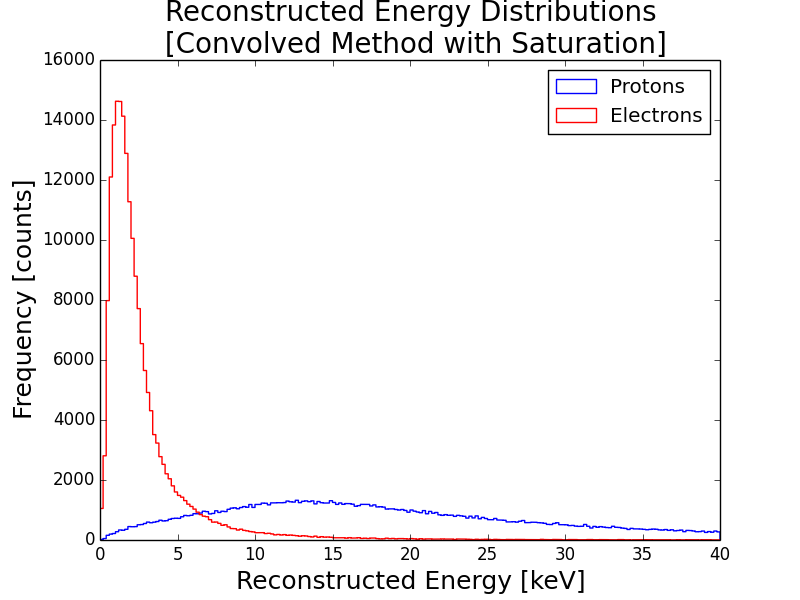
\includegraphics[scale=0.5]{Images2/convolvedSat.png}
    \caption{Reconstructed Energies using truncated fit method.}
    \label{fig:recoEnergyFunc4}
\end{figure} 

This improvement in the fit model can also be seen in the frequency plot of the reconstructed energies (shown in Figure \ref{fig:recoEnergyFunc4}). This is further validated by the corresponding purity-efficiency curve in Figure \ref{fig:rejectionPlot}.

These distributions match those of the corresponding MC energy distribution (Figure \ref{mcenergydistributions}) much more closely than the convolved fit without truncation. In particular, the distributions agree well beyond the 3 keV region, allowing us to recover much of the dynamic range of the ADC. 

In addition, note that this model will be key when fitting cross talk data in which the waveforms will have a similar shape but the reconstructed energies will occur at energies much closer to electrons.
(Should I delete this sentence???)


\section{Multi-peak Methods}
By utilizing the convolution fit method with truncation, the vast majority of data is fit with great accuracy. This final addition, will serve to address a small fraction of hits.


%Consider the frequency histogram (Figure \ref{initialSigmaDistribution}) for the fitting parameter $\sigma$ of the convolved fit. 

%\begin{figure}[htp!]
%    \centering
%    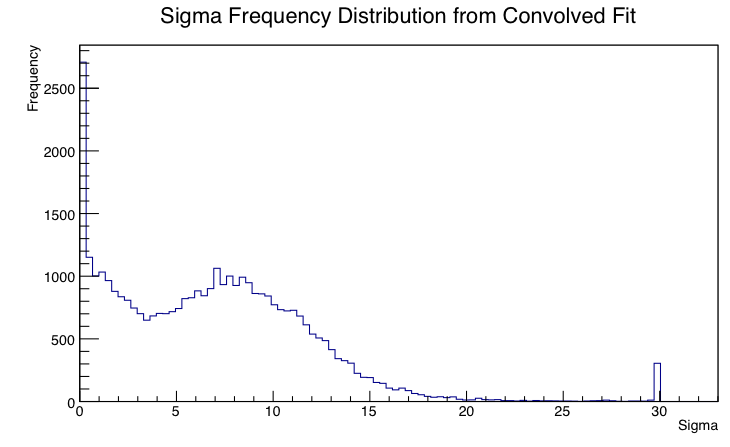
\includegraphics[width=0.7\textwidth]{Images/initialSigmaDistribution.png}
%    \caption{Frequency distribution for the fitting parameter $\sigma$ from the convolved fit.}
%    \label{initialSigmaDistribution}
%\end{figure} 

%It appears that the majority of values are centered around $15$ while falling mainly in the range of $0$ to $25$. In addition, there are two peaks, one at $0$ and one at $30$. The fits with $\sigma = 0$ are fits in which the charge a hit was deposited on the wire approximately instantaneously. Therefore, this peak is physically meaningful and warrants no concern. The peak at $\sigma = 30$ is a consequence of the fact that a limit of $30$ was placed on the fit parameter. Consequently, this peak actually corresponds to a tail reaching beyond $30$, and upon inspection consists of poor fits.




For many of these fits the output appears to be a superposition of multiple waveforms occuring within the same 240 ns period. To further explore this an explicit peak search was applied to the data. A distribution of the number of peaks found is shown in Figure \ref{fig:peakSearch}. From this figure, we can see that roughly five percent of hits recorded contain more than one peak. Two methods are used to address this possibility.

\begin{figure}[htp!]
    \centering
    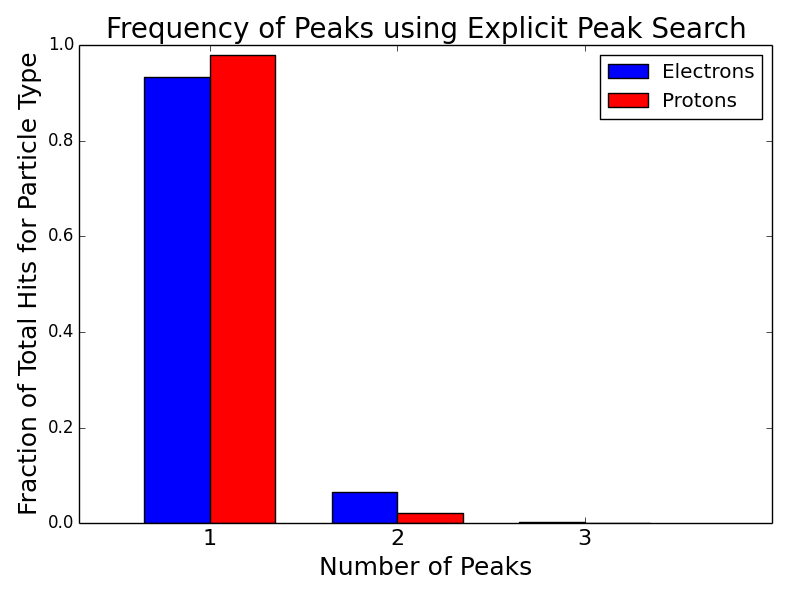
\includegraphics[width=0.7\textwidth]{Images2/peakSearch.png}
    \caption{Distribution of peaks found using explicit peak search.}
    \label{fig:peakSearch}
\end{figure} 


\subsection{Early Peak Method}

 One possibility for a double peak hit is that the primary hit for the 240 ns period is superimposed on a previous waveform which has not sufficiently decayed. Since the end of a waveform can be well-approximated by an exponential decay, a term of the form $Q(t) = e^{-t / \tau}$ can be added to the fit function. A sample fit is shown in Figure \ref{fig:earlyPeak}.

  %This additional approximately exponential decay, can force the fitted value of the pedestal to be overestimated which results in a event which can not be well-fitted by a simple convoluted fit. To address this issue an approximate solution to the decay of a waveform $Q(t) = e^{-t / \tau}$ can be added to the fit function. 
  %As can be seen in the sample fit, this solution appears to be succesful, and reduces several of the high sigma values.  

\begin{figure}[htp!]
    \centering
    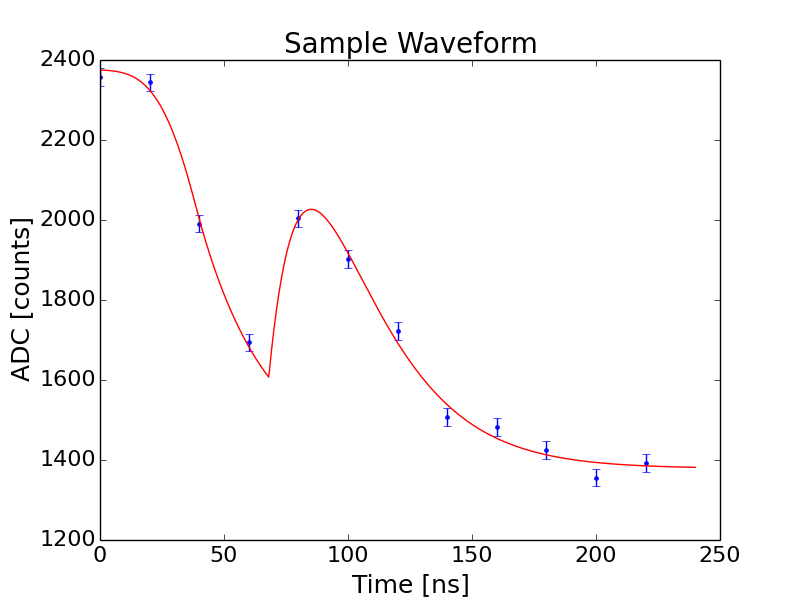
\includegraphics[scale=0.6]{Images2/dynamicPed.png}
    \caption{Sample waveform fitted with early peak method.}
    \label{fig:earlyPeak}
\end{figure} 
%A plot of the reconstructed energies for the protons and electrons is shown in Figure \ref{recoEnergyFunc7}. Note that there is not a significant change in the distributions with respect to the corresponding plot using the truncated fit method.



\subsection{Late Peak Method}

A double peak hit can also occur when a secondary hit occurs shortly after the primary hit. To model this, two of the base convolved fits can be summed together. To speed up the fitting process and to control the complexity of the fit model, the convolution parameter of $\sigma$ for both hits are fixed to $7$ ns. Thus, there are five free parameters in the fit. Note that the value of $7$ is fairly arbitrary, but has been found to be fairly reasonable. (Should I refer to sigma distribution here?)


%To reduce the number of free parameters



%Note that we cannot use two convolved fits, since we do not have enough information for each hit ($8$ samples - $8$ fit parameters = $0$ degrees of freedom). In addition, note that by using the baseline fit, we have assumed a value of $\sigma = 0$ for each peak. However, from \ref{initialSigmaDistribution} another option might be to use two convolved fits with $\sigma$ fixed to 8.

%Adjusting the fit parameters so that the two peaks can not overlap significantly, we are able to achieve a relatively successful fit. Note that this fit is only successful for fits which contain two peaks. Therefore, its use must be restricted to certain cases. Hence, this fit is only effective when used alongside the convolved fit with a dynamic pedestal. 

\begin{figure}[htp!]
    \centering
    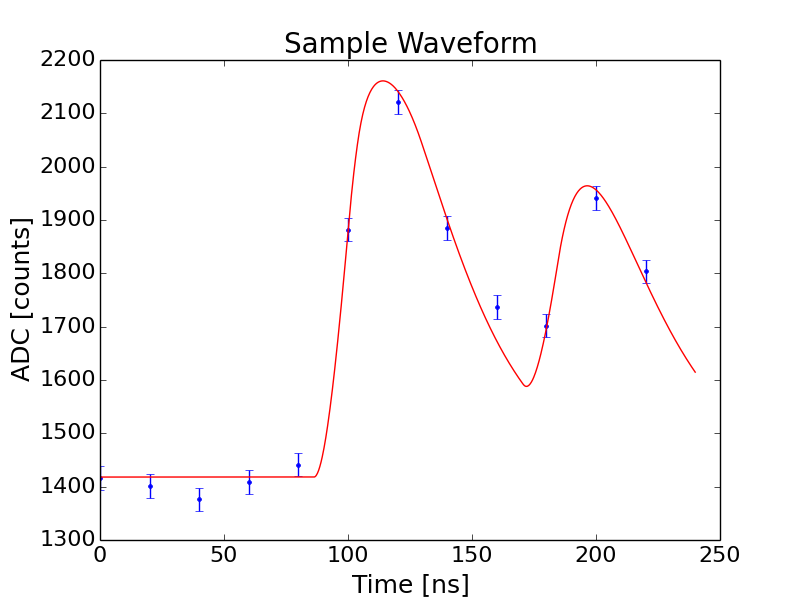
\includegraphics[width=0.6\textwidth]{Images2/double.png}
    \caption{Sample waveform fitted with late peak method.}
\end{figure} 

\begin{figure}[htp!]
    \centering
    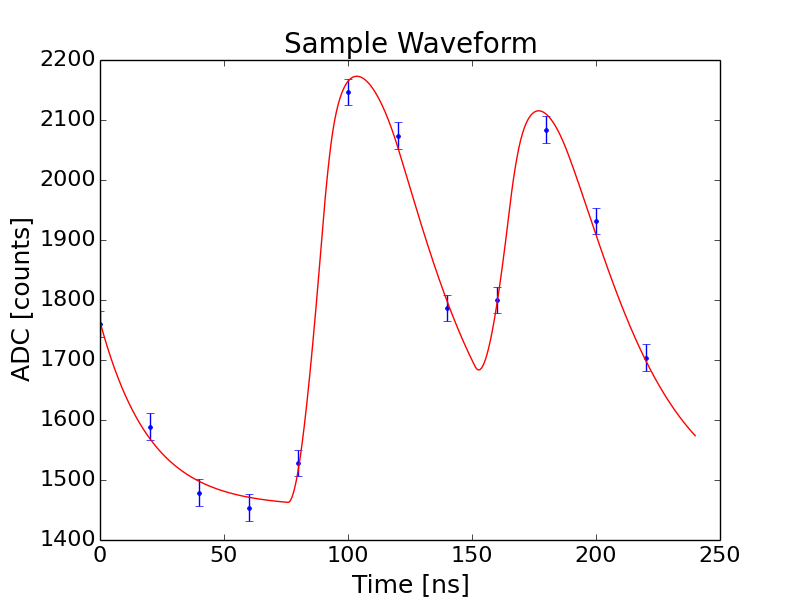
\includegraphics[width=0.6\textwidth]{Images2/full.png}
    \caption{Sample fit with both an early peak and a late peak.}
    \label{fig:full}
\end{figure} 

\subsection{Early and Late Peak Method}
For completion, note that in Figure \ref{fig:peakSearch}, there are a small subset of hits in which three peaks are found. These cases can be fit to a model which contains both an early and a late peak. A sample fit is shown in Figure \ref{fig:full}.



\subsection{Triage Method}
In summary, by first applying an explicit peak search, 
we can determine the number and approximate locations of peaks over for each given 240 ns interval. With this information, we can determine whether to use a convolved fit or a multi-peak fit method. Note that determining whether the secondary peak is an early peak is extremely simple : simply 

%To determine whether to use the double peak fit method or the convolved fit method with the dynamic pedestal the following algorithm has been used: if the chisquare value from the dynamic pedestal method is at least three times greater than the chisquare value for the double peak fit method, use the dynamic pedestal method. Otherwise, use the double peak fit method. Note that this algorithm for differentiating the waveforms has not yet been optimized.

Using this algorithm, energy distributions for electrons and protons can be reproduced (Figure ). Note that this plot closely resembles Figure \ref{fig:recoEnergyFunc4} since the addition of the triage only effects the analysis of roughly 5 percent of hits.

\begin{figure}[htp!]
    \centering
    \makebox[0pt]{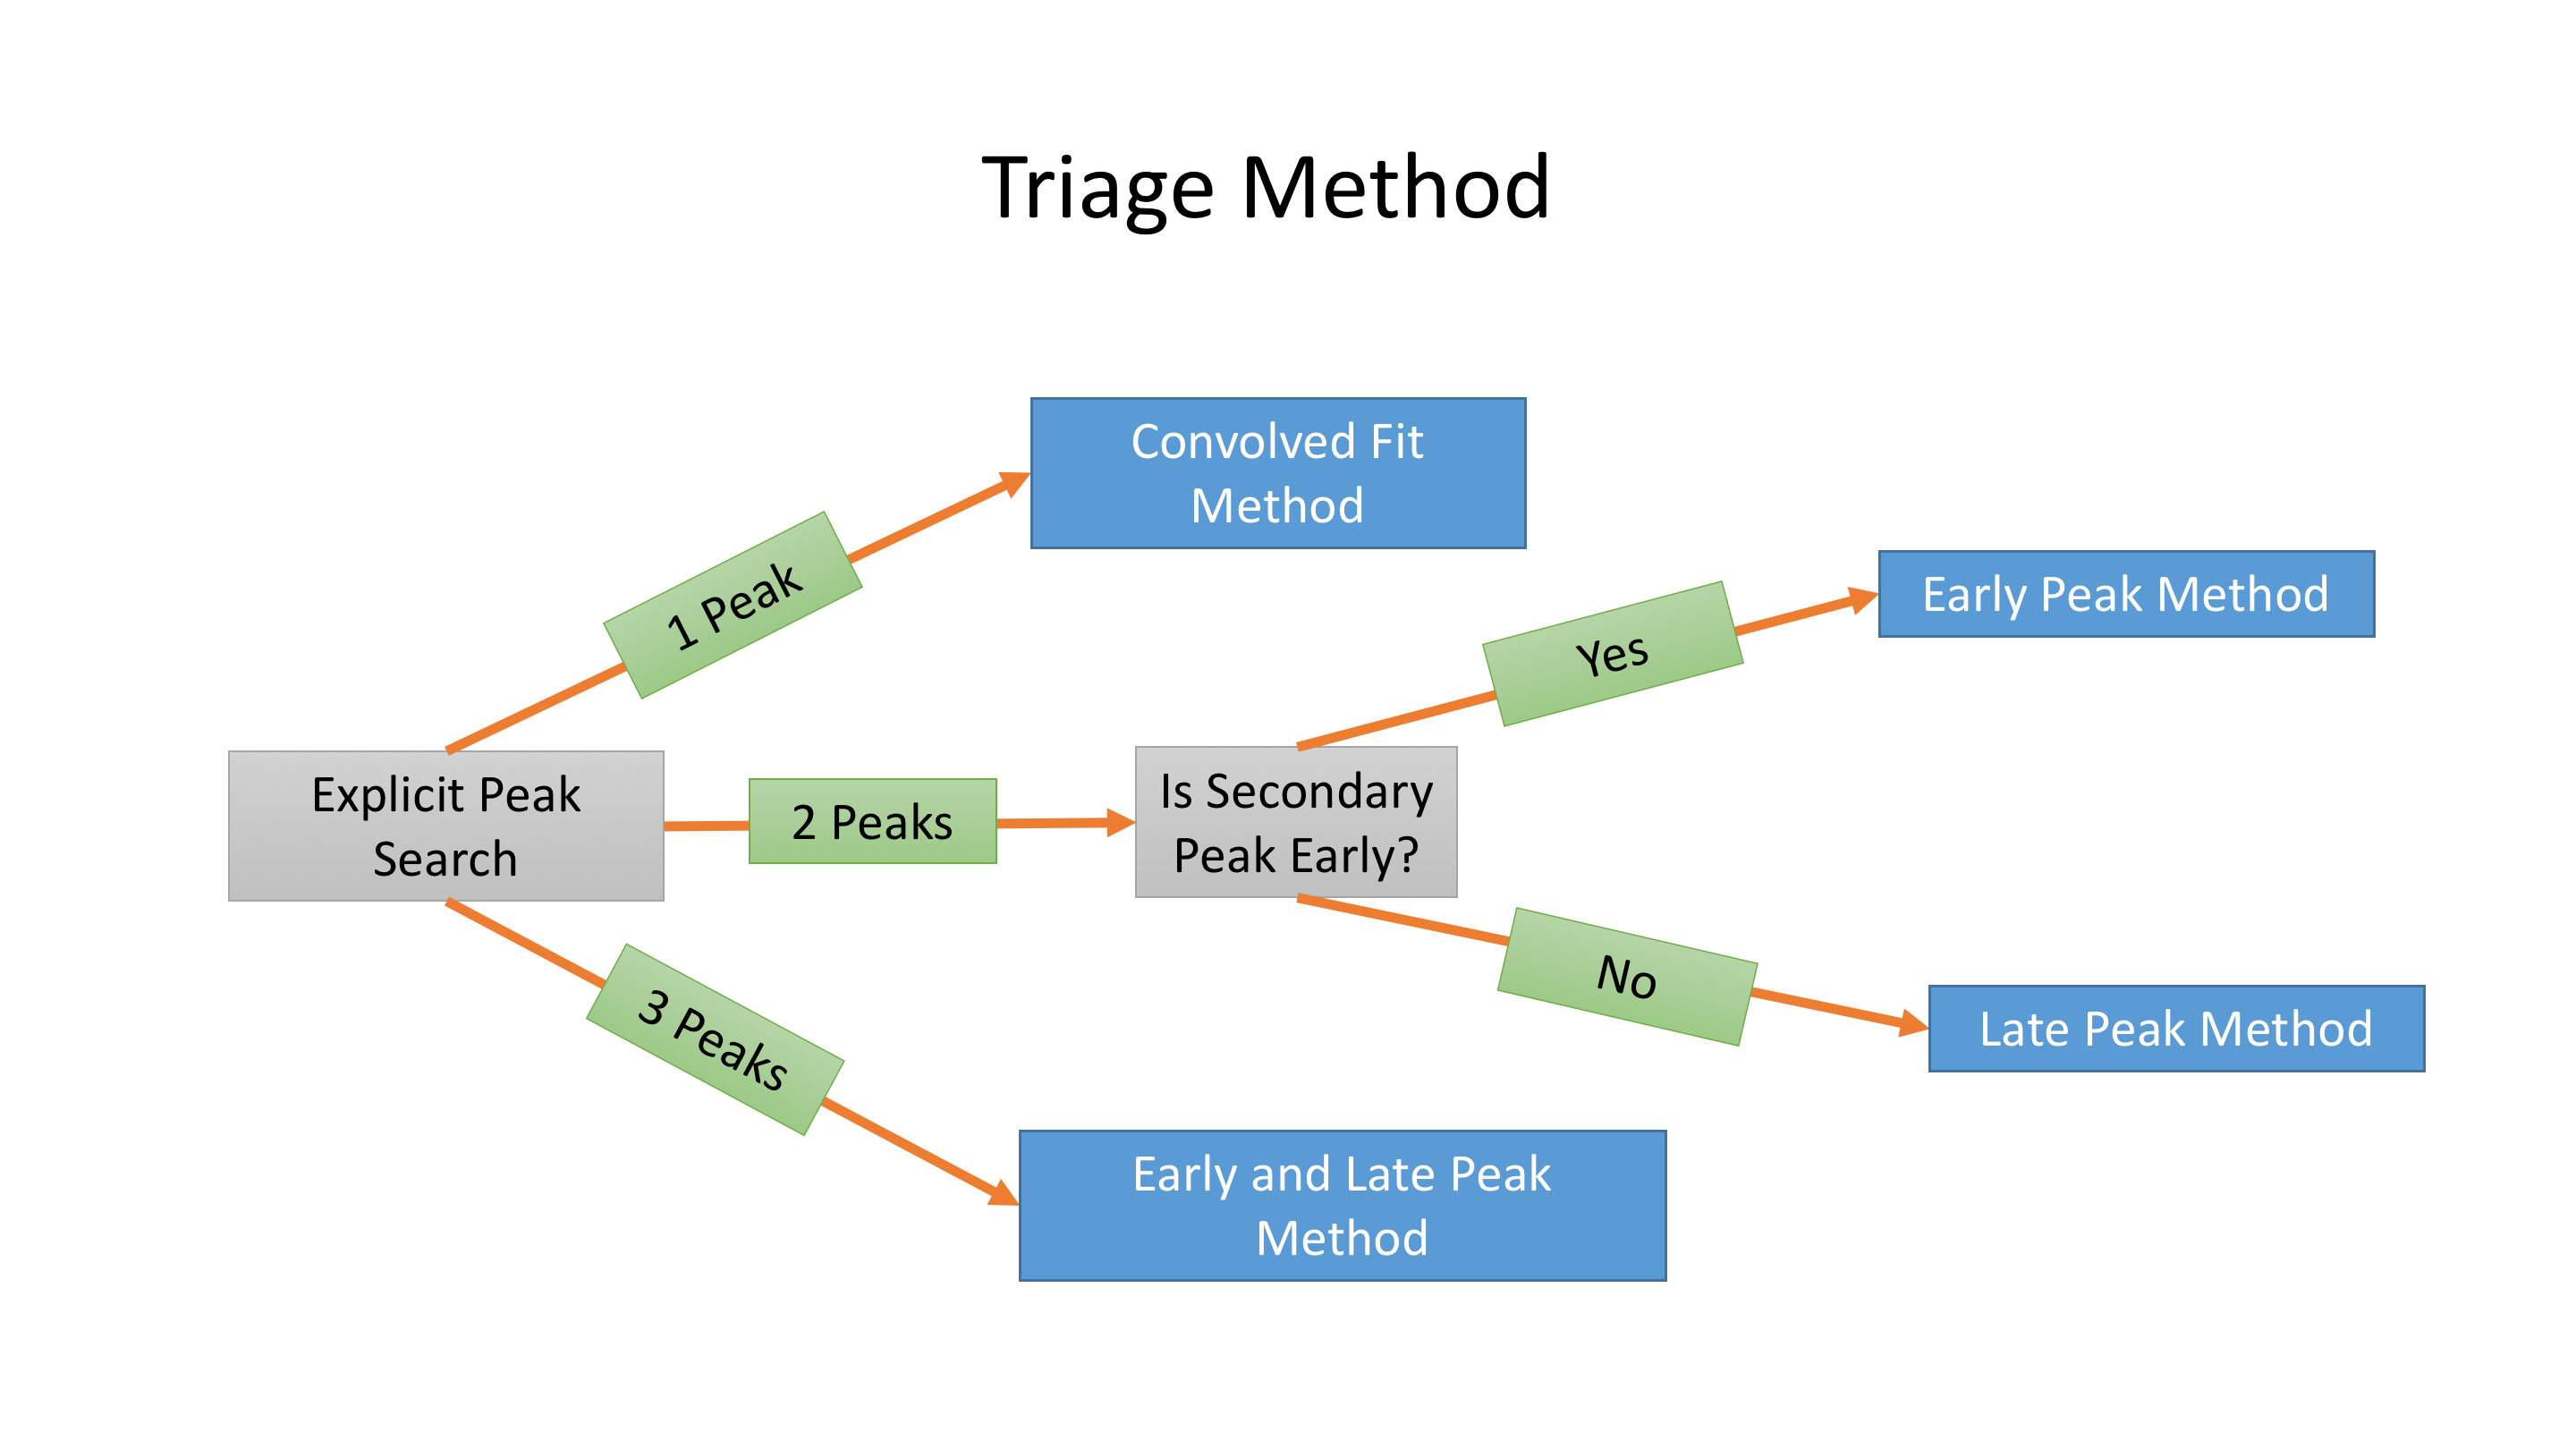
\includegraphics[scale=0.4]{Images2/triageMethod.png}}
    \caption{Decision processes used in triage method.}
    \label{fig:triage}
\end{figure} 



\begin{figure}[htp!]
    \centering
    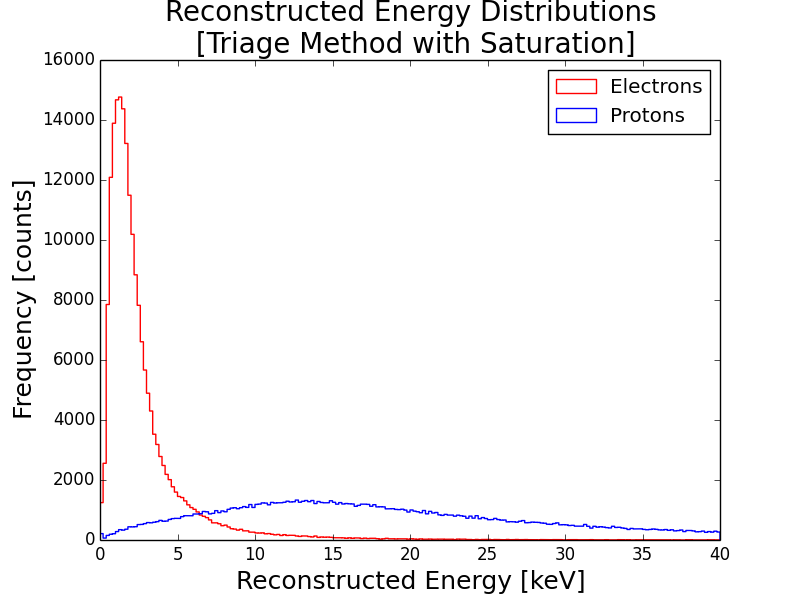
\includegraphics[width=0.6\textwidth]{Images2/triage.png}
    \caption{Reconstructed Energies using triage method with truncation.}
    \label{fig:triage}
\end{figure} 

%After utilizing this algorithm, the distribution of the parameter $\sigma$ has been reproduced (Figure \ref{finalSigmaDistribution}). Note that, all fits corresponding to double peaks (as determined from the algorithm in the previous paragraph) have been removed. 
%\begin{figure}[htp!]
%    \centering
%    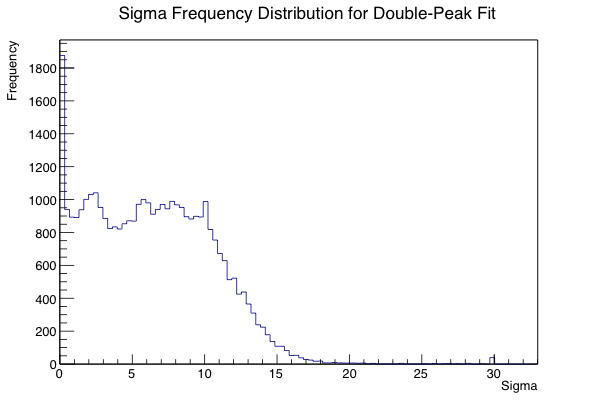
\includegraphics[width=0.55\textwidth]{Images/finalSigmaDistribution.png}
%    \caption{Computed energy from ADC versus MC energy. Note that the energy from the ADC has been roughly scaled to units of MeV.}
%    \label{finalSigmaDistribution}
%\end{figure} 

%Clearly, this method is successful in eliminating the tail in the sigma distribution.

%Lastly, for comparison consider the frequency plot of the reconstructed energies of the protons and electrons (Figure \ref{recoEnergyFunc8}). No significant changes can be seen in the distributions for the two particles.


\begin{figure}[htp!]
    \centering
    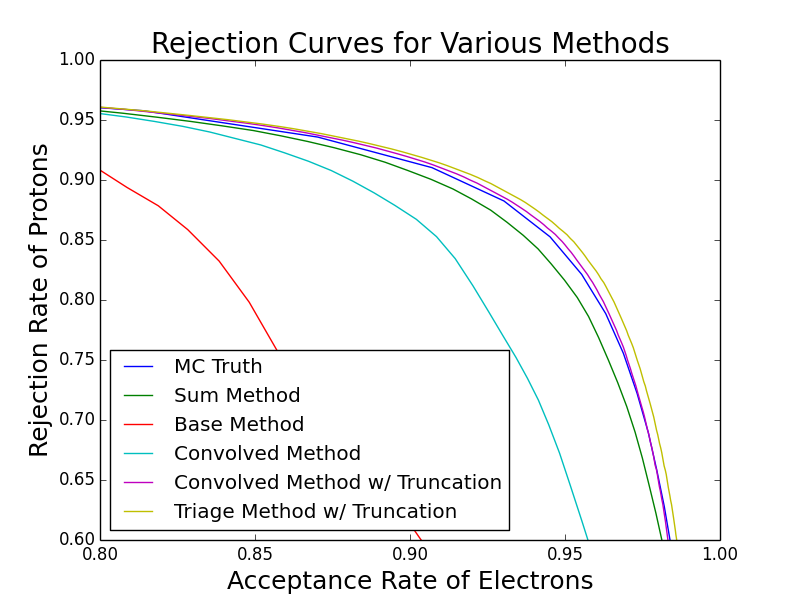
\includegraphics[scale=0.6]{Images2/rejectAll.png}
    \caption{Reconstructed Energies using triage method with truncation.}
    \label{fig:rejectionPlot}
\end{figure} 


\section{Results} 

As described at the beginning of this chapter, the figure of merit is the comparison of the rejection curves for the various methods, which is presented in Figure \ref{fig:rejectionPlot}.

The base fit method and convolved fit methods perform worse than the sum method. However, by introducing the convolved and saturation models, the fit method performs significantly better. In fact, it performs better than differentiation using the MC energy. This makes sense, since even without triage, the convolved fit method will sometimes fit to the primary peak even if other peaks appear in the waveform.

Lastly, it is clear that the triage method performs the best.  In the range relevant to the Mu2e experiment (which corresponds to an approximately a 95\% acceptance rate of electrons), the triage fit method has rejects over 22 percent of proton hits accepted by the sum method.

 %approximately an 1\% improvement over the sum method. In particular, the double peak method performs the best as it can differentiate double particles while the MC energy can not. Note that the double peak fit method will likely perform better in the actual experiment, since less double peak hits appeared in the data used than would be expected. (This is a result of a compromise made in order to measure more high energy electron hits. This effect will be removed in future studies.)



 %\[ f(v_{in}) =  \left\{
 %       \begin{array}{ll}
 %           v_{in} & \quad v_{in} \leq v_{sat} \\
 %           v_{max} - (v_{max} - v_{sat}) e^{-\frac{v_{in} - v_{sat}}{v_{max} - v_{sat}}} & \quad v_{in} > v_{sat}
  %      \end{array}
  %  \right.
%\] 


 % Discussion of subdivision surfaces for m-rep boundaries
                              % sec:subdivproximity
                              % Section on proximity tests for subdivision boundaries
                              % sec:subdivmedialinterp
                              % Section on medial interpolation of subdivision solids
%ch:conclusion
%!TEX root = AllegThesis.tex
%
% $Id: conclusion.tex
%

\chapter{Discussion and Future Work}\label{ch:conclusion}

%This chapter should contain the following items, though not
%necessarily in this order or sectioned this way in particular.

%\section{A discussion of the significance of the results}

%\section{A review of claims and contributions}


%\section{Future work}

%\section{Final words}
 % Chapter on DS-Surfaces:  Boundary Displacments and Texturing
                              %   and on Multifigure Modeling of M-rep Subdivision Solids


%\appendix
%%
% $Id: appa.tex,v 1.1 1999/11/19 23:21:25 culver Exp $
%

\chapter{Here's the first appendix---these are optional}\label{ch:appa}

Limit positions and tangent vectors (and thus normals) can be computed for initial
even vertices of a subdivision mesh by weighted averages of their local
n-neighborhood with appropriately computed masks.

\section{Limit positions for regular, valence-4
vertices}\label{chsec:regular4vertex}

\section{Blah blah blah}

Blah blah blah.
              % Appendix A---Limit Positions for Catmull-Clark Surfaces
%%
% $Id: appb.tex,v 1.1 1999/11/19 23:21:25 culver Exp $
%
\chapter{Here's a second appendix}\label{ch:appb}

\begin{quote}
\small ``When I have nothing to say, my lips are sealed.  Say something once,
why say it again?"
---David Byrne.
\end{quote}

\section{Put something here}

\section{Put something here}
              % Appendix B---Inverting Limit Positions for Irregular Meshes

%\nocite{ckm-acmap-99}
%\nocite{Dierckx93}
%\nocite{obs-stcav-92}
%\nocite{bb4471}

%\nocite{*} includes all BibTeX references in the bibliography
% COMMENT THIS OUT FOR YOUR FINAL VERSION
\nocite{*}

\begin{spacing}{1}
  \bibliographystyle{plain}
  \bibliography{Bibdir/myBibtexDB}
\end{spacing}

%%
% $Id: colophon.tex,v 1.1 1999/11/19 23:21:27 culver Exp $
%

\begin{colophon}
  This thesis was typeset using the \LaTeXe{} typesetting system with the
  gatorthesis.sty style file.  Figures were drawn using xfig on a Linux box,
exported to .eps, and cropped to a good bounding box by Ghostview on a PC by running
PS-to-EPS.

\end{colophon}


\typeout{THEPAGE \thepage}

\end{document}
